\documentclass[color=black,11pt]{elegantpaper}
\usepackage{amsfonts} 
\usepackage{makecell} 
\usepackage{hyperref}
\usepackage{mathdots}
%\usepackage{makeindex}
%\makeindex
\title{Real numbers.}
%\subtitle{Foundation of calculus}

\author{Sergey Nikitin}
%\institute{Elegant\LaTeX{} Program}
\date{January 20,2025}
\version{1.0}
%\bioinfo{Bio}{Information}


%\logo{spinning-calc.png}
%\cover{DSCF1445.JPG}

% modify the color in the middle of titlepage
\definecolor{customcolor}{RGB}{32,178,170}
\colorlet{coverlinecolor}{customcolor}

\begin{document}

\maketitle

%\frontmatter
%\tableofcontents

%\mainmatter
\section*{Nihil est sine ratione. There is nothing without a reason.\\
                         Gottfried Leibniz }
\begin{abstract}
	The paper describes the construction of numeral systems out of the given alphabet and the set of meta symbols. The presentation starts with binary alphabet $\{0,\;1\}.$ Then it continues with the ternary numeral system. Along the way it also shows the significance of Euclid and Euler-Fermat algorithms. Then it illustrates Euler-Fermat algorithm during the discussion of the most popular on our planet numeral system based on the set of westernized Arabic numerals, $\{0,\;1,\;2,\;3,\;4,\;5,\;6,\;7,\;8,\;9\}.$ The fundamental topological properties of real numbers conclude this paper.
\end{abstract}	
%%%%%%%%%%%%%%%%%introduction
\phantomsection
%\addcontentsline{toc}{chapter}{Introduction}
\section*{Introduction}
%\paragraph{Why another one? }
There are many calculus textbooks. If your institution burdens you with requirement to have one for your class then try to save  money by renting it, buying a subscription to a web-site with its digital version, and/or purchasing a used one. With a few exceptions, all calculus textbooks cover more or less the same pool of ideas that are dated back to $17$th - $19$th centuries. They also thoroughly preserve some misrepresentations,  delusions and lack of knowledge that were acceptable a while ago but now not only look ridiculous but also might create serious obstacles to primary consumers of calculus: future engineers, physicists, mathematicians to name a few. One of the aims of this text is to free reader from debilitating side effects of traditional education as far as calculus is concerned. The reader is not required to have any special mathematical background in order to break free from the iron chains of memorized rules and antique traditions and discover free world of mathematical ideas.\\


%\paragraph{ Framework}
 
   Real numbers are constructed as names for points on a straight line. The names are created out of a finite alphabet supplemented with meta-symbols. That was done more than four thousand years ago by one of early human civilizations. Then it was repeated numerous times over centuries across the planet with different alphabets and meta-symbols. Our contemporary understanding of real numbers was coined at the end of 19th and the beginning of 20th century. Unfortunately current University courses assume that the students already know and understand real numbers and either ignore this topic completely or shadow its content with the set of formal axioms. This manuscript does not require any prior knowledge of numbers. In fact, you could be completely clueless about them. We build real numbers from scratch by starting with binary numeral system (alphabet $\{0,\;1\}),$  then continuing with ternary system (alphabet $\{0,1,2\})$ and introducing the Cantor set along the way. After completing the first two sections the reader will be able to create a  numeral system  out of any given alphabet. For this reason our presentation of building decimal numeral system out of Arabic numerals $\{0,1,2,3,4,5,6,7,8,9\}$ is a bit sketchy because the main purpose there is to illustrate the ideas of P. Fermat and L. Euler (17th-18th century). Little Fermat's theorem (17th century) and its Euler's enhancement (18th century)  allow us to prove that\\
\begin{center}
\begin{itshape}
 A real number is a ratio of two integers if, and only if, its name is either a finite word or a periodic tail sequence.
\end{itshape}
\end{center} 
This statement does not care about our alphabet choice. It is valid in all numeral systems. We also present a new proof of Euler's theorem. Our proof does not use the group theory as it is usually done in traditional texts on number theory and algebra. Instead it's main tool is Euler-Fermat's algorithm that not only allows us to prove Euler's enhancement of little Fermat's theorem but also efficiently calculates periods of ratios. The manuscript has numerous examples that illustrate applications of Euler-Fermat's algorithm. Moreover, Euler-Fermat's algorithm admits simple computer implementation ( see the source code of \href{https://github.com/mathhobbit/EditCalculateAndChart}{EditCalculateAndChart} in GitHub.)\\ 
Section ~\ref{sec:Cardinality} also describes Cantor's diagonalization idea. It implies that real numbers are uncountable. Anything bijective to real numbers is called continuum. It also leads us to Cantor's continuum hypothesis. 
\begin{center}
\begin{itshape}
The smallest uncountable set is continuum.
\end{itshape}
\end{center}
This proposition awaits its proof or a counter example that will break it. Chapter  ~\ref{ch:real_numbers} ends with the discussion on metric and topological properties of real numbers. In particular, we prove that the set of real numbers is a complete metric space.

Happy reading!!!\\
Sergey Nikitin 
 
%%%%%%%%%%%%%%%%%%%done with introduction

%\chapter{Real numbers}
\section{Binary numeral system.} 
\label{sec:binary}

Our first goal is to come up with names for points on a straight line. Each point on the straight line should have its own unique name. Each name will be constructed out of the symbols from a fixed alphabet. For simplicity we start with the alphabet that consists of two symbols: $0 \;\;\mbox{ and }\;\; 1.$ Let us choose an arbitrary point on the straight line and name it $0.$ Now our straight line looks as shown on Fig. \ref{fig:only_zero}. 

\begin{figure}[htbp]
  \centering
  \includegraphics[width=0.6\textwidth]{xfig_stuff/straight_line_with0.eps}
  \caption{All points are nameless but $0.$}
  \label{fig:only_zero}
\end{figure}

We have one more symbol left. It is $1.$  We choose another point and call it $1.$  On the planet earth, in the current version of human civilization, the point with name $1$ is chosen on the right of $0$ point. However, there is nothing wrong to put it on the left of $0.$  There is no surprise if it was or will be done on another planet or in some other version of human civilization. Putting $1$ on the left or right of $0$ introduces the order among the symbols of our alphabet. This book is written on the planet Earth at the beginning of 21st century CE, therefor $1$ goes to the right of $0.$ We are saying that $0$ is smaller than $1$ and writing $0<1$ (Fig.~\ref{fig:zero_and_1}). We also can express it by saying: 
\begin{itemize}
\item $0$ is on the left of $1;$
\item $1$ is on the right of $0.$
\end{itemize}
It makes no difference whatsoever. I like  $0<1.$ It is shorter.
\begin{figure}[htbp]
  \centering
  \includegraphics[width=0.6\textwidth]{xfig_stuff/Line_with_0_and_1.eps}
  \caption{$0$ is on the left of $1,$ therefore $0<1.$}
  \label{fig:zero_and_1}
\end{figure}
In order to create names for other points we need to use various combinations of symbols from our alphabet $\{0,\;1\}.$ All combinations of symbols from alphabet $\{0,\;1\}$ are either words (finite number of symbols) or sequences (infinite number of symbols) made of $\{0,\;1\}.$

Symbol $0$ occupies a special place in our alphabet. In particular, all wards and the sequence of zeroes 
$$
0,\;00,\;000,\; \dots
$$
will identify the single point $0.$ Consider all combinations that start with $1.$ Since $0<1$ we can order them \href{https://en.wikipedia.org/wiki/Lexicographic_order}{lexicographically} (like words in a dictionary). The list written in ascending lexicographical order looks as follows.
$$
1,\;10,\;11,\;100,\;101,\;110,\;111,\;1000,\;1001,\;1010,\;\dots
$$ 

Now we are ready to name new points on the straight line. For that purpose we will use a measuring stick equal to the distance between $0$ and $1.$ With this measuring stick we put the next point with name $10$ on the right of $1$. Then the next $11$ on the right of $10$. Then $100.$ Continuing in this manner we name quite a few points on the straight line (Fig. ~\ref{fig:natural_numbers}). 

\begin{figure}[htbp]
  \centering
  \includegraphics[width=0.6\textwidth]{xfig_stuff/Line_with_natural_numbers.eps}
  \caption{Points with names $0,\;1,\;10,\;11,\;\dots$}
  \label{fig:natural_numbers}
\end{figure}
Each name represents a distance between $0$ and the respective point. For example, $1$ is the distance from $0$ to $1$ (one measuring stick), $10$ is the distance from $0$ to $10$ (two measuring sticks) etc. We can introduce addition,  subtraction,  multiplication and division operations on the set of names made of $\{0,\;1 \}$ in the same way as reader probably learned playing with measuring sticks in elementary school or preschool (if not then please take a break from reading go and play with measuring sticks and then come back). This set of names, each starting with $1,$
$$
1,\;10,\;11,\;100,\;101,\;110,\;111,\;1000,\;1001,\;1010,\;\dots
$$
is called \href{https://en.wikipedia.org/wiki/Natural_number}{natural numbers} and denoted by $\mathbb{N}.$ In addition to the alphabet $\{0,\;1\}$ we need meta-symbols $\{+,\;-,\;\cdot,\;/ ,\; . \}.$ 
\begin{itemize}
\item $a \cdot b$ is product (the result of multiplication) of $a$ and $b;$
\item $a+b$ is addition;
\item $a-b$ subtraction;
\item $a / b$ division;
\item the last meta-symbol, the point, will be used to build new names. 
\end{itemize}
Historically, natural numbers $\mathbb{N}$ were probably one of the first mathematical abstractions discovered by humans.  The main characteristic of natural numbers is that they contain a starting element $1$ and all other elements are obtained from $1$ by applying a measuring stick. Formally speaking $\mathbb{N}$ is the smallest set of numbers with the following two properties.
\begin{itemize}
\item[1.] It contains $1$
\item[2.] Together with $n$ it also contains $n+1 .$ 
\end{itemize}
It leads us to the principle of \href{https://en.wikipedia.org/wiki/Mathematical_induction}{mathematical induction}. If you want to prove that some statement $S$ is true for all $n\in \mathbb{N}$ then you do it in two steps.
\begin{itemize} 
\item[1.]{\bf Foundation step.} Check that $S$ is true for $n=1.$ 
\item[2.]{\bf Induction step.} Assume that $S$ is true for $n$  then prove that $S$ is also true for $n+1.$ 
\end{itemize}
 

For points on the left of $0$ we preserve the same names but use prefix "-". Now our straight line looks as shown on Fig. ~\ref{fig:line_with_integers}.
\begin{figure}[htbp]
  \centering
  \includegraphics[width=0.6\textwidth]{xfig_stuff/Line_with_integers.eps}
  \caption{Integers}
  \label{fig:line_with_integers}
\end{figure}
This set of numbers ($0$ is included now) is called integers and denoted by $\mathbb{Z}.$

We still have many nameless points. They are all sitting between neighboring integers in the intervals constructed with our measuring stick.  Let us first name points between $0$ and $1.$ We include $0$ and exclude $1.$ This set of points is denoted by $[0,\;1).$
Notice that our alphabet is
$$
\{0,\;1\}\;\;\mbox{ and } \;\; 0 < 1
$$
Suppose we need to name a point {\bf \color{red}a} (Fig. ~\ref{fig:point_between_0_and_1}). We divide the interval $[0,1)$ into two equal parts. The first part is called $0$, the second $1.$
\begin{figure}[htbp]
  \centering
  \includegraphics[width=0.6\textwidth]{xfig_stuff/ZeroInterval.eps}
  \caption{$0$ is the first letter of the name for $a.$}
  \label{fig:point_between_0_and_1}
\end{figure}
Our point {\bf \color{red}a} is located in the $0$ interval. We set $0$ as the first letter of its name. Then we repeat the procedure by dividing the $0$ interval into two equal parts and calling them $0$ and $1$ respectively (Fig. ~\ref{fig:2nd_letter_choice}).
\begin{figure}[htbp]
  \centering
  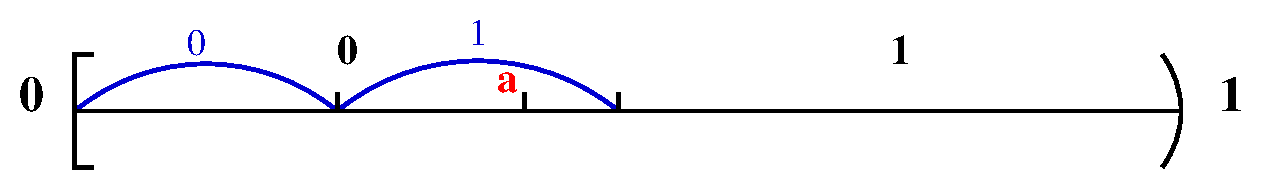
\includegraphics[width=0.6\textwidth]{xfig_stuff/2ndLetterInTheName.eps}
  \caption{$1$ is the second letter of the name for $a.$}
  \label{fig:2nd_letter_choice}
\end{figure}
Our point {\bf \color{red}a} is located in the $1$ sub-interval of $0$ part of $[0,\;1)$ (sounds like gibberish if you do not look at the pictures). To choose the subsequent letters we repeat our procedure again and again. If at one of the steps (during the division of the respective interval into two equal parts) we hit our point $a,$ then we put $1$ and  the naming procedure is finished (look at the local address in ~\ref{fig:globallocaladdress}). {\bf \color{red}a} has a finite length name (a word made of $\{0,\;1\}.).$ If we never hit {\bf \color{red}a} in the course of our algorithm then the name for {\bf \color{red}a} will have infinitely many letters from our alphabet (the name is a sequence made of $\{0,\;1\})$ (Fig. ~\ref{fig:complete_address_a}).

We can apply the described naming algorithm for any interval between neighboring natural numbers (non-negative integers) and come up with local names for points. In order to make them unique we will prepend the local names for the points with the name of the respective interval. The name of the interval is the natural number at its left boundary. For example, the interval $[0,\;1)$ has the name $0.$ The interval $[10,\;11)$ has the name "$10$" etc. The global address of a point (the name of the interval) and the local address (local name inside the interval) are written next to each other and separated by a meta-symbol (in this book, it is the point (Fig. ~\ref{fig:complete_address_a} and Fig. ~\ref{fig:globallocaladdress})).\\ 

We constructed names out of the alphabet $\{0,\;1\}$ for all points from the straight line that are located on the right of zero.\\
\begin{figure}[htbp]
  \centering
  \includegraphics[width=0.6\textwidth]{xfig_stuff/CompleteAddress.eps}
  \caption{$a = 0.0110\dots$}
  \label{fig:complete_address_a}
\end{figure}
For example, the point with name $100.11$ has local address $11$ in the interval with name $100$ (see Fig.~\ref{fig:globallocaladdress}). 
\begin{figure}[htbp]
  \centering
  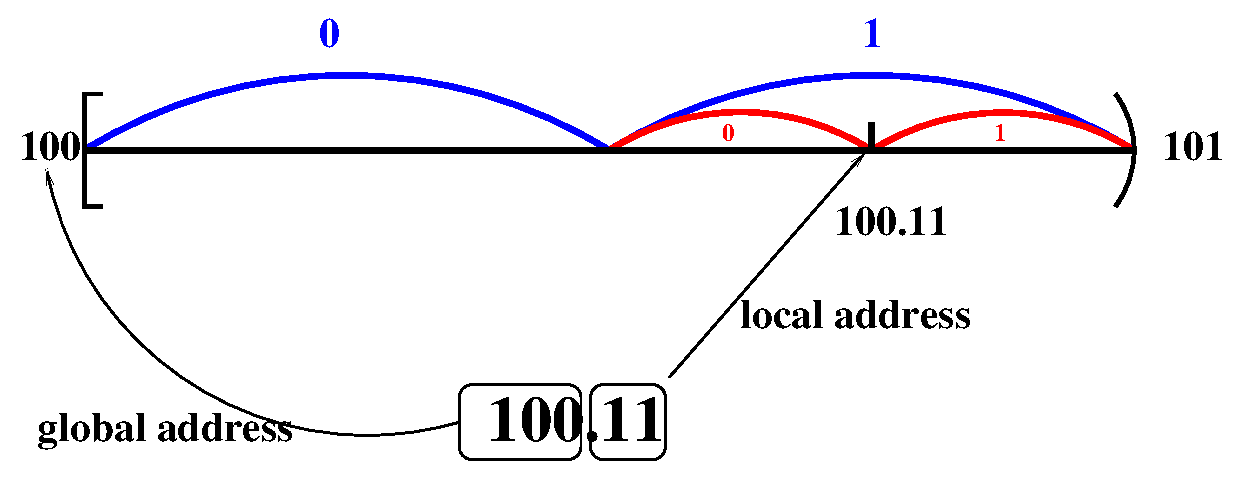
\includegraphics[width=0.6\textwidth]{xfig_stuff/globallocaladdress.eps}
  \caption{Global address is 100, local 11.}
  \label{fig:globallocaladdress}
\end{figure}
 Names for points on the left of zero are constructed in the way which is sort of a mirror image of what we did for points on the right of zero. In particular, for negative points we consider intervals $(-(j+1),-j]\;\;( j>0)$ and the name for the interval (global address) is its right end, $-j $ (instead of a left end for the points on the right of zero). For example, the interval $(-1,0]$ has the name "$0$". The interval $(-11,-10]$ has the name "$-10$" etc. The negative local addresses coincide with names for points from the interval $(-1,0].$ The algorithm for writing negative local addresses is a mirror image of what we did for points from $[0,\;1)$ depicted on Fig. ~\ref{fig:point_between_0_and_1}, Fig. ~\ref{fig:2nd_letter_choice} and Fig. ~\ref{fig:complete_address_a}. 
\begin{center}
\begin{picture}(60,1)
\thicklines
\put(0,0){\line(1,0){60}}
\end{picture}
\end{center}
\begin{example}
Write a binary representation for $-\frac{4}{3} .$ The ratio $-\frac{4}{3}$ belongs to the interval $(-2,\;-1]$. Therefore its global address is $-1$ and its local address inside the interval $(-2,\; -1]$ coincides with the local address of $-\frac{1}{3}$ from $(-1,\;0].$ To make it brief,
$$
-\frac{4}{3} = -1 - \frac{1}{3}
$$ 
In order to calculate the binary representation for $-\frac{1}{3}$ we split the interval $(-1,\;0]$ into two equal parts. We name the left part $1$ and the right part $0$ (Fig. ~\ref{fig:point_on_the_left}). The ratio $- \frac{1}{3}$ belong to the part with name $0.$ The first letter of its local address is $0.$ Then we split the interval with name $0$ into two equal parts (the left part is called $1$, the right $0$) and repeat the procedure.

\begin{figure}[htbp]
  \centering
  \includegraphics[width=0.6\textwidth]{xfig_stuff/rypoint_on_the_left.eps}
  \caption{The binary representation of $-\frac{1}{3}$ is $-0.\overline{01}$}
  \label{fig:point_on_the_left}
\end{figure}

 After several steps of the algorithm we can observe that the binary representation for $-\frac{4}{3} $ is the sequence
$$
-1.01010101\dots
$$
with periodic tail. The period is $01.$ This is written as
$$
-1.\overline{01}
$$ 
One can see it also as follows.
$$
-\frac{1}{3} = -\frac{1}{2^2-1}= -\frac{1}{2^2}\cdot \frac{1}{1-\frac{1}{2^2}}=-\frac{0 \cdot 2 + 1}{2^2}\sum_{j=0}^{\infty} (\frac{1}{2^2})^j
$$
This idea will be developed in section ~\ref{sec:ratio_are} of this manuscript.
\end{example}
\begin{center}
\begin{picture}(60,1)
\thicklines
\put(0,0){\line(1,0){60}}
\end{picture}
\end{center}
The constructed naming convention is called a numeral (and/or numerical) system.
A numeral system is always based on an alphabet. The number of letters in the alphabet is called \href{https://en.wikipedia.org/wiki/Radix}{radix} of the numeral system. In other words, we constructed a numeral system of radix $2.$ Sometimes it is also called binary system. Points of the straight line correspond to real numbers. The set of real numbers is denoted by $\mathbb{R}.$\\


In addition to natural numbers $\mathbb{N},$  integers $\mathbb{Z}$ and real numbers $\mathbb{R}$ there is the set of rational numbers (quotients) defined as
$$
\mathbb{Q} = \{ m/n\;;\; m,\;n \in \mathbb{Z}\;\mbox{ and } n \not= 0 \}
$$
The set of rational numbers contains $\mathbb{Z}$ and is smaller than $\mathbb{R},$
$$
\mathbb{N} \subset \mathbb{Z} \subset \mathbb{Q}  \subset \mathbb{R}.
$$ 
The achievements of this section can be summarized in a purely mathematical form.
\begin{theorem}
Any positive real number $A \in \mathbb{R}$ can be represented as follows. There exist $M \in \mathbb{N}$ such that
$$
 A \;=\; \sum_{m= 0}^M a_m \cdot 2^m + \sum_{n > 0}b_n \frac{1}{2^n} 
$$
where each $a_m$ and each $b_n$ is equal either $0$ or $1,$ and  the second sum can be either finite or infinite. The record 
$$
A = a_M \; a_{M-1}\; \dots a_0\;.\;b_1\; b_2 \;\dots 
$$
is called a binary representation of $A.$
\end{theorem}
Any negative $A_{-} \in \mathbb{R}$ is a mirror image of some positive $A_{+} \in \mathbb{R}$ and we have
$$
 A_{-}\; =\; -A_{+} \;=\;- (\sum_{m= 0}^M a_m \cdot 2^m + \sum_{n > 0}b_n \frac{1}{2^n}).
$$
Sometimes our naming convention is also referred to as the positional numeral system of base (instead or radix) $2.$  For any integer $B$ one can construct the numeral system of base (radix) $B.$ In particular, now-days the most popular numeral system has radix $10.$ Regardless of radix, all positional numeral systems have some defect (everybody knows about this shortcoming but silently ignores it). Let us briefly discuss it using binary system as example. 

The problem is that names for rational numbers represented by words are not unique in any numeral system regardless of its radix (base). In fact each rational number represented by a word has two completely different names that are both valid. For example,
$$
1 = 0.111 \dots 111 \dots
$$  
The word $1$ and the sequence of $1$'s identify the same point. Irrational numbers (those that are not in $\mathbb{Q})$ do not have this problem. Also there is no problem with names for  rational numbers represented by sequences having periodic tails with periods different from $1$ (in binary numeral system). Later on we will prove that a number is rational if, and only if, it can be represented either by a word or by a sequence with a periodic tail. One of the possible ways to overcome this non-uniqueness of names is to  demand for all numbers to be represented by sequences. That means all names that are words we will replace by the respective sequences (with the tail of $1$'s in binary system). However, it is not good for various applications (in particular for computer arithmetic) because, in real world, we use words not sequences. A periodic sequence is also fine in applications as long as its period is not humongous. In this book we will show an innocent elementary school problems that can lead to sequences having tails with huge periods that can baffle into distraction any digital device on this planet. The reasonable revision of naming convention is to demand for each name to be of minimal possible length. That will also make each name unique and it is well suited for various applications. Anyway, the reader please beware that ghosts of unknown are always around you, right around the corner (not necessary a dark one).

\section{Ternary numeral system. Cantor set.}
\label{sec:ternary}
A ternary numeral system has radix $3.$  It uses alphabet $\{0,\;1,\;2\}.$  We pick the first arbitrary point and call it $0.$ We use a measuring stick and mark the point on the right of $0$ as $1.$ One measuring stick to the right of $1$ we put point $2.$ Our line looks now as shown on Fig. ~\ref{fig:3points}.
\begin{figure}[htbp]
  \centering
  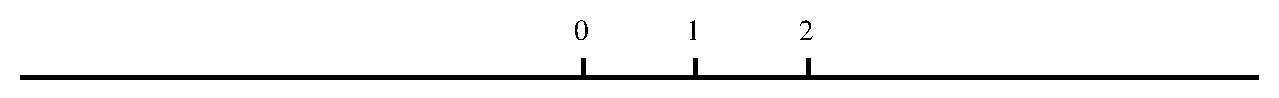
\includegraphics[width=0.6\textwidth]{xfig_stuff/3points.eps}
  \caption{Ternary numeral system, $\{0,\;1,\;2\}.$} 
  \label{fig:3points}
\end{figure}
It introduces order in our alphabet
$$
\{0,\;1,\;2\}, \;\;0<1,\;\;1<2
$$
Consider all combinations of symbols from $\{0,\;1,\;2\}$  that start either with $1$ or $2.$ We can write them in ascending lexicographical order as follows.
$$
1,\; 2, \; 10,\; 11, \; 12, \;20, \; 21, \; 22,\; 100,\; 101,\;102,\; \dots
$$
Those are the names of the points on the right of $0.$ Each point obtained from the previous by applying a measuring stick (Fig. ~\ref{fig:3natural}).

\begin{figure}[htbp]
  \centering
  \includegraphics[width=0.6\textwidth]{xfig_stuff/3natural.eps}
  \caption{Ternary representation of $\mathbb{N}.$} 
  \label{fig:3natural}
\end{figure}

 This is the ternary representation of natural numbers $\mathbb{N}.$ For points on the left of $0$ we use the same names only prepend them with the metasymbol "$-$". All those names including $0$ give us the ternary representation of integers $\mathbb{Z}$ (Fig. ~\ref{fig:3integers}).
\begin{figure}[htbp]
  \centering
  \includegraphics[width=0.6\textwidth]{xfig_stuff/3integers.eps}
  \caption{Ternary representation of $\mathbb{Z}.$} 
  \label{fig:3integers}
\end{figure}
We can introduce operations addition, subtraction, multiplication, division in a natural way (playing with measuring sticks).
The name of a point located between two consecutive non-negative integers $i$ and $i+1$ consists of two parts. The first part (global address) is the name of the interval $i$ (the left end of $[i,\; i+1)$ if $i>0).$ The second part is the local address, the position of the point inside $[i,\;i+1).$ 
To calculate a local address in a ternary numeral system for a point {\bf \color{red} a} from the interval $[0,\;1)$ we divide the interval into three equal parts (Fig. ~\ref{fig:3ZeroInterval}) (number of parts is equal to the radix of the numeral system). The first letter in the local address of {\bf \color{red} a} is the name of the interval that contains {\bf \color{red} a}.
\begin{figure}[htbp]
  \centering
  \includegraphics[width=0.6\textwidth]{xfig_stuff/3ZeroInterval.eps}
  \caption{$1$ is the first letter of the local address for {\bf \color{red} a}.} 
  \label{fig:3ZeroInterval}
\end{figure}
In this examples it is $1.$ We repeat this procedure for the interval with name $1.$ We divide it into tree equal subintervals with names $0,\;\;1$ and $2$ and choose the next letter for the local address of {\bf \color{red} a} (Fig. ~\ref{fig:3ZeroIntervalWith1Subdivided}).
\begin{figure}[htbp]
  \centering
  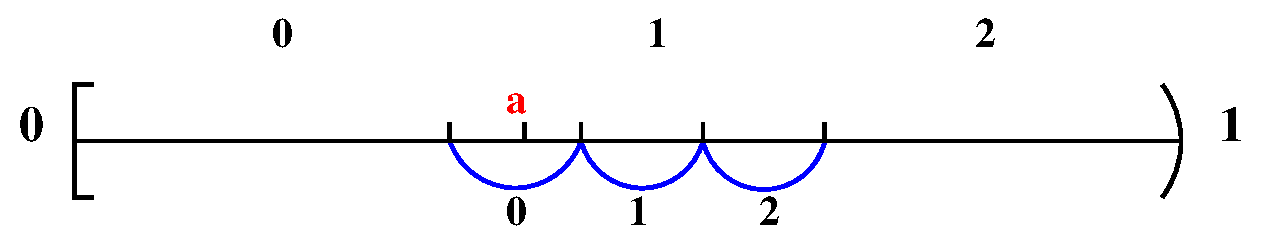
\includegraphics[width=0.6\textwidth]{xfig_stuff/3ZeroIntervalWith1Subdivided.eps}
  \caption{{\bf \color{red} a}$=0.10\dots.$} 
  \label{fig:3ZeroIntervalWith1Subdivided}
\end{figure}
If at some step we hit point {\bf \color{red} a} during subdividing an interval into three equal parts then we write the letter corresponding to the interval on the right of {\bf \color{red} a} and stop. The local address for {\bf \color{red} a} will be a finite word written in the alphabet of $\{0,\;1,\;2\}.$ Otherwise, the name for {\bf \color{red} a} is a sequence of symbols from $\{0,\;1,\;2\}.$\\

In order to write names for points on the left of zero we mirror the operations that we did for points on the right of zero. Namely, the name of the interval (global address) $(-(j+1),\;-j]\;\;(j>0)$ is its right end (instead of left), $-j.$ Negative local addresses coincide with the local addresses from $(-1,\;0]$ derived by mirroring the steps we did when writing names for points from $[0,\;1).$ \\

\begin{center}
\begin{picture}(60,1)
\thicklines
\put(0,0){\line(1,0){60}}
\end{picture}
\end{center}
\begin{example}
Write a ternary representation for $-\frac{9}{5} .$ The ratio $-\frac{9}{5}$ belongs to the interval $(-2,\;-1]$. Therefore its global address is $-1$ and its local address inside the interval $(-2,\; -1]$ coincides with the local address of $-\frac{4}{5}$ from $(-1,\;0].$ To make it brief,
$$
-\frac{9}{5} = -1 - \frac{4}{5}
$$ 
In order to calculate the binary representation for $-\frac{4}{5}$ we split the interval $(-1,\;0]$ into three equal parts. We name the left part $2,$ the middle $1$ and the right part $0.$ The quotient $-\frac{4}{5}$ belong to the interval with name $2.$ Hence, the first letter of its local address is $2.$ Splitting the interval with name $2$ into three equal parts and repeating the procedure yields $1$ as the next letter of the local address for $-\frac{4}{5}.$ Continuing with application of this algorithm we come to the conclusion that the ternary representation for $-\frac{9}{5} $ is the following sequence with a periodic tail.
$$
-1.\overline{2101}
$$
One can see it also as follows.
$$
\frac{4}{5} = \frac{4\cdot 16}{5 \cdot 16} = \frac{64}{3^4- 1}=\frac{2\cdot 3^3+1\cdot 3^2+0\cdot 3 + 1}{3^4- 1}=\frac{2\cdot 3^3+1\cdot 3^2+0\cdot 3 + 1 }{3^4}\sum_{j=0}^{\infty} (\frac{1}{3^4})^j
$$
As you can see the ternary period for $-\frac{9}{5}$ is $2101.$  In section ~\ref{sec:ratio_are} we will extend this idea to calculating a period for a fraction in a numeral system with an arbitrary radix.

\end{example}
\begin{center}
\begin{picture}(60,1)
\thicklines
\put(0,0){\line(1,0){60}}
\end{picture}
\end{center}
All local ternary addresses of points on $[0,\;1)$ are words and sequences written in alphabet $\{0,\;1,\;2\}.$

\begin{definition}(\href{https://en.wikipedia.org/wiki/Cantor_set}{Cantor set})\\
The subset of points from $[0,\;1)$ with local ternary addresses written only with letters $0$ and $2$ ($1$ is excluded) is called Cantor set.
\end{definition}
Cantor set was discovered in 19th century. It has some peculiar properties. In order to describe them we need some mathematical machinery that will be developed in the next section.\\
The construction of ternary numeral system leads us to the following conclusion.
\begin{theorem}
Any positive real number $A \in \mathbb{R}$ can be represented as follows. There exist $M \in \mathbb{N}$ such that
$$
 A \;=\; \sum_{m= 0}^M a_m \cdot 3^m + \sum_{n > 0}b_n \frac{1}{3^n} 
$$
where each $a_m$ and each $b_n$ can be one of the following symbols:  $0,\;1,\;2.$  The second sum can be either finite or infinite. The record 
$$
A = a_M \; a_{M-1}\; \dots a_0\;.\;b_1\; b_2 \;\dots 
$$
is called a ternary representation of $A.$
\end{theorem}
For negative $A \in \mathbb{R}$ we have
$$
 A \;=\;- (\sum_{m= 0}^M a_m \cdot 3^m + \sum_{n > 0}b_n \frac{1}{3^n}).
$$



%\section{\href{https://en.wikipedia.org/wiki/Cardinality}{Cardinality.} \href{https://en.wikipedia.org/wiki/Cantor's_diagonal_argument}{Cantor's diagonalization.} \href{https://en.wikipedia.org/wiki/Continuum_hypothesis}{Continuum hypothesis.}}   
\section{\href{https://en.wikipedia.org/wiki/Function_(mathematics)}{Functions.} \href{https://en.wikipedia.org/wiki/Injective_function}{Injections}, \href{https://en.wikipedia.org/wiki/Surjective_function}{surjections} and \href{https://en.wikipedia.org/wiki/Bijection}{bijections.}}
Let $A$ and $B$ be arbitrary sets of elements. Consider a mapping
$$
f:\;A\;\to \; B
$$
The domain $D_f$ of the mapping $f$ is the set of elements $x\in A$ where $f(x)$ is defined.
$$
D_f = \{ x\in A;\; f(x) \mbox{ makes some sense } \}
$$ 
Clearly $D_f$ is a subset of $A.$ It is denoted by 
$$
D_f \subset A
$$
 The range $R_f$ of $f$ is a subset of $B.$ $R_f$ consists of $y \in B$ such that there exists $x \in A$ and $y = f(x).$ We can present this statement in a concise form with the help of \href{https://en.wikipedia.org/wiki/Quantifier_(logic)}{quantifiers},
\begin{eqnarray*}
\exists && \mbox{  means "there exist(s)" }\\
\forall && \mbox{ means "for all" } \nonumber
\end{eqnarray*}
Now in terms of quantifiers it looks as follows
$$
R_f = \{y \in B;\;\exists x \in A \mbox{ such that } y = f(x) \}
$$ 
A mapping $y = f(x),$
$$
f:\;A\;\to \; B
$$
is called a \href{https://en.wikipedia.org/wiki/Function_(mathematics)}{function} if one-to-many relationship between $x$ and $y=f(x)$ is not allowed. In other words, for any $x \in D_f \subset  A$ there exists the only $y \in R_f \subset B$ such that $y = f(x)$ (Fig. ~\ref{fig:ConceptOfFunction}).

\begin{figure}[htbp]
  \centering
  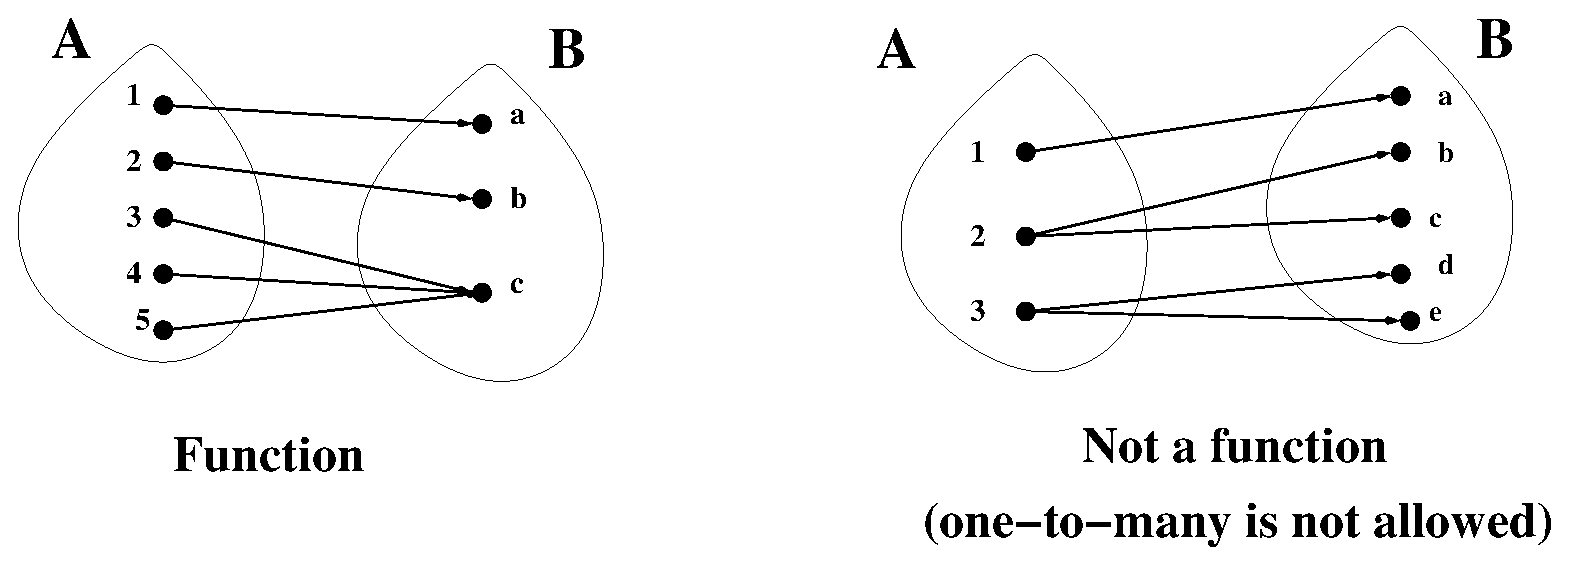
\includegraphics[width=0.6\textwidth]{xfig_stuff/ConceptOfAFunction.eps}
  \caption{One-to-many is illegal for a mapping that wants to be a function.} 
  \label{fig:ConceptOfFunction}
\end{figure}
Functions are mappings with one-to-many relationship out of question. There are also different types of functions.

\begin{definition}
\href{https://en.wikipedia.org/wiki/Injective_function}{An injective function or an injection} is a function
$$
f:\;A\;\to \; B
$$
such that
$$
D_f = A
$$
and 
$$
\forall\;x_1,\; x_2 \in A\;\;x_1 \; \not=\; x_2 \implies f(x_1) \not= f(x_2).
$$
\end{definition}
 An injection sticks $A$ into the inside of $B$ in one-to-one manner (Fig.~\ref{fig:injection}). The next type of functions covers the whole $B$ with some part of $A$ (Fig. ~\ref{fig:surjection}).
\begin{figure}[htbp]
  \centering
  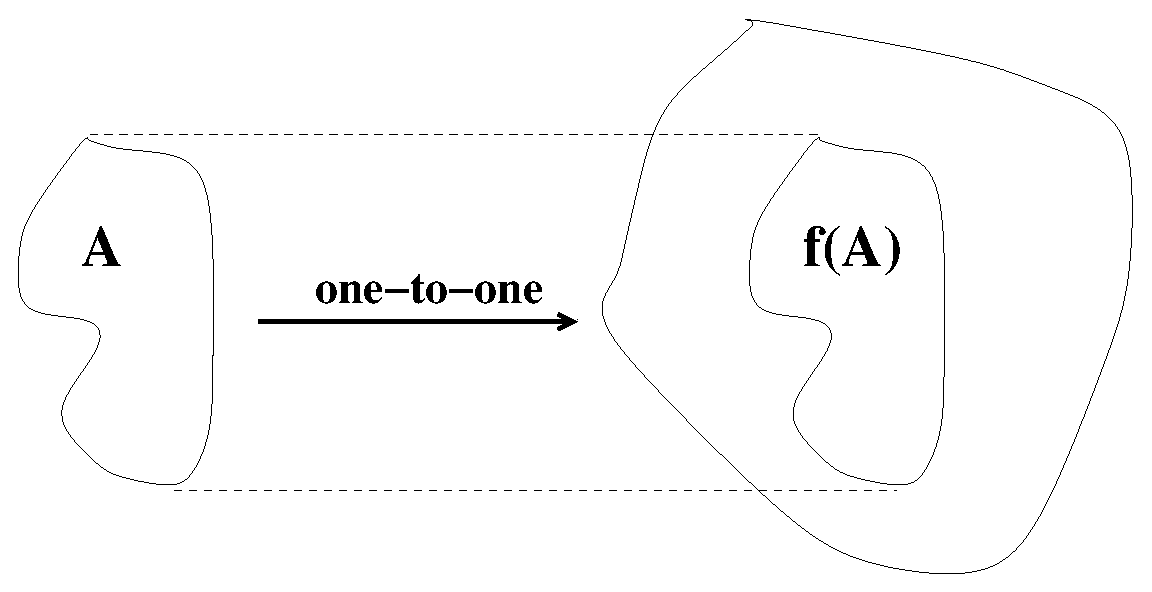
\includegraphics[width=0.6\textwidth]{xfig_stuff/injection.eps}
  \caption{An injection $f:\;A \to B$ is a one-to-one function $f:\;A\to f(A)\subset B$ } 
  \label{fig:injection}
\end{figure}
\begin{definition}
\href{https://en.wikipedia.org/wiki/Surjective_function}{A surjective function or a surjection} is a function
$$
f:\;A\;\to \; B
$$
such that
$$
\forall \;y \in B\;\;\exists\;x \in A\;\;\mbox{ such that } f(x)=y.
$$
\end{definition}
\begin{figure}[htbp]
  \centering
  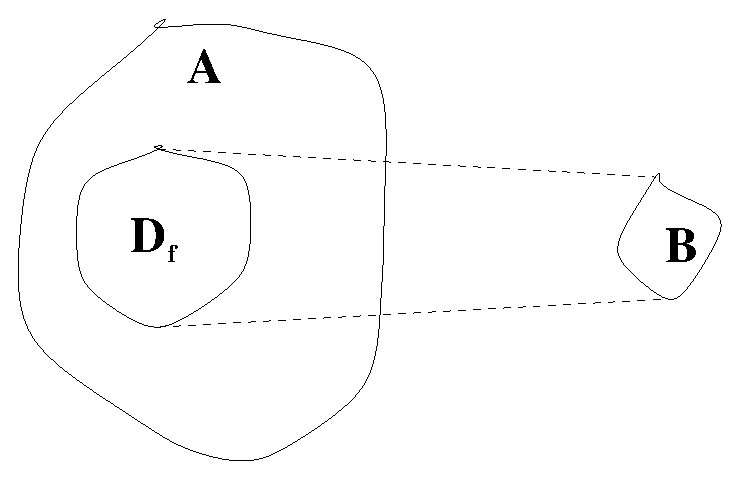
\includegraphics[width=0.6\textwidth]{xfig_stuff/surjection.eps}
  \caption{A surjection $f:\;A \to B$ is a surjection $f:\;D_f\to B,$ where $D_f \subset A$ }  
  \label{fig:surjection}
\end{figure}
A function 
$$
f:\;A \to B
$$
which is both injection and surjection of $A$ onto $B$ is called \href{https://en.wikipedia.org/wiki/Bijection}{bijection.}

\begin{definition}
\href{https://en.wikipedia.org/wiki/Bijection#:~:text=In%20mathematics%2C%20a%20bijection%2C%20also,with%20exactly%20one%20element%20of}{A bijective function or a bijection} is a function
$$
f:\;A\;\to \; B
$$
such that
$$
\forall\;x_1,\; x_2 \in A\;\;x_1 \; \not=\; x_2 \implies f(x_1) \not= f(x_2).
$$
and
$$
\forall \;y \in B\;\;\exists\;x \in A\;\;\mbox{ such that } f(x)=y.
$$
\end{definition}
A bijection is also called a one-to-one function. A bijection 
$$
f:\;A\to B
$$
has the inverse function
$$
f^{-1} :\; B \to A
$$
which is also a bijection and
$$
f(f^{-1}(y)) = y \;\;\mbox{ and }\;\;f^{-1}(f(x))=x
$$
for any $x\in A$ and $y \in B.$

%$\aleph_0$

\section{\href{https://en.wikipedia.org/wiki/Cardinality}{Cardinality.} ~\href{https://en.wikipedia.org/wiki/Cantor's_diagonal_argumenT}{Cantor diagonal trick and continuum.} }
\label{sec:Cardinality}
Cardinality or a cardinal number is the number of elements in a finite set. If the set $A$ is infinite then its cardinality represents the collection of the sets that are bijective to $A.$
\begin{definition}
Any two sets $A$ and $B$ are said to have the same cardinalities or the same cardinal numbers if, and only if, there exists a bijection
$$
f :\; A \to B
$$
It is denoted as $card(A) = card(B),$ where $card(A)$ and $card(B)$ are cardinals numbers of $A$ and $B$ respectively.
\end{definition}
Natural numbers $\mathbb{N}$ comprise of cardinalities of finite sets. The smallest infinite set is $\mathbb{N}.$ Its cardinality is called \href{https://en.wikipedia.org/wiki/Aleph_number}{aleph-null} and denoted by $\aleph_0.$ A set $A$ of cardinality $\aleph_0$ is called countable. Its elements can be counted and the set $A$ can be written as a sequence
$$
a_1,\;a_2,\;a_3,\;a_4,\; \dots
$$
where $a_j \in A$ for $j=1,\;2,\;3,\;4,\;\dots.$ In other words, There exists a bijection
$$
f:\;\mathbb{N} \to A
$$
such that
$$
\forall\; j\in \mathbb{N}\;\;f(j)= a_j
$$
and
$$
\forall \; a \in A \; \exists j\in \mathbb{N} \;\;\mbox{ such that } a = a_j\;\;\mbox{ or } f(j) = a.
$$
For any natural number $n \in \mathbb{N}$ of countable sets
$$
A_1,\;A_2,\;\dots ,\; A_n
$$
their union
$$
\bigcup_{i = 1}^n A_i 
$$
is also countable. We can prove this statement by writing those sets as sequences next to each other,
\begin{eqnarray*}
A_1 &=& \{a_{11},\;a_{12},\;a_{13},\; \dots \}\\
A_2 &=& \{a_{21},\;a_{22},\;a_{23},\; \dots \}\\
A_3 &=& \{a_{31},\;a_{32},\;a_{33},\; \dots \}\\
\vdots \\
A_n &=& \{a_{n1},\;a_{n2},\;a_{n3},\; \dots \}
\end{eqnarray*} 
Then we write
$$
\{ a_{ij}\}_{i+j=m} \;\;\mbox{ for } m=2,\;3,\;4,\;\dots
$$
next to each other in lexicographical order of the indices for $a_{ij}.$ It looks as follows.
$$
a_{11},\; a_{12},\;a_{21},\;a_{13},\;a_{22},\;a_{31},\;\dots
$$
Thus
$$
\bigcup_{i = 1}^n A_i 
$$
can be written as a sequence. Therefore it is countable or has cardinality $\aleph_0.$ The same method depicted in (Fig. ~\ref{fig:countable}) proves that
$$
\bigcup_{i = 1}^\infty A_i
$$
has cardinality $\aleph_0$ or is countable.
\begin{figure}[htbp]
  \centering
  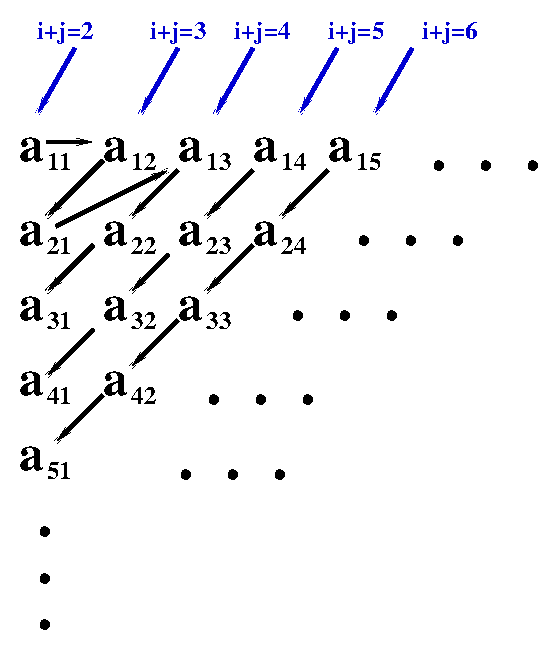
\includegraphics[width=6cm, height=7cm]{xfig_stuff/Countable.eps}
  \caption{Countable union of countable sets is countable}
  \label{fig:countable}
\end{figure}

Natural numbers $\mathbb{N},$ integers $\mathbb{Z},$ quotients $\mathbb{Q}$ are all of cardinality $\aleph_0 .$ However, the set of real numbers $\mathbb{R}$ is a different animal. 

$\mathbb{R}$ is not countable. In order to prove it we rely on \href{https://en.wikipedia.org/wiki/Georg_Cantor}{G. Cantor} diagonalization trick.

By reductio ad absurdum let us assume that $\mathbb{R}$ is countable. Then we can use binary numeral system and write local addresses for points from $[0,\;1]$ as a sequence
$$
a_1,\;a_2,\;a_3,\;a_4,\; \dots
$$
where each $a_j (j=1,\; 2,\; 3,\;4,\; \dots)$ is a sequence
$$
a_j = a_{j1},\;a_{j2},\;a_{j3},\;a_{j4}, \; \dots
$$
 of letters from the alphabet $\{0,\;1\};$ each $a{ij}$ is either $0$ or $1 (i,j=1,\;2,\;3,\;\dots ).$ 

By assumption all points from $[0,\;1)$ are listed as rows from the following table.
\begin{eqnarray*}
&& a_{11},\;a_{12},\;a_{13},\;a_{14}, \; \dots\\
&& a_{21},\;a_{22},\;a_{23},\;a_{24}, \; \dots\\
&& a_{31},\;a_{32},\;a_{33},\;a_{34}, \; \dots\\
&& a_{41},\;a_{42},\;a_{43},\;a_{44}, \; \dots\\
&& \vdots
\end{eqnarray*}
Here comes \href{https://en.wikipedia.org/wiki/Cantor%27s_diagonal_argument}{the diagonal trick} by G. Cantor. Consider a point $b$ defined by 
$$
b=b_1,\;b_2,\; b_3,\; \dots
$$  
where 
$$
b_j=\left\{\begin{array}{ccc}
           0& \mbox{ for } & a_{jj} =1\\
           1& \mbox{ for } & a_{jj} =0\\
          \end{array} 
    \right. 
$$
By construction $b$ does not belong to our table. At the same time $b$ is a name for a point from $[0,\;1].$ It contradicts to the assumption that all points from $[0,1]$ are in our table.\\
 The set $[0,1]$ is not countable. Its cardinality is denoted by aleph-one, $\aleph_1.$  A set of cardinality $\aleph_1$ is called continuum. Each row
$$
a_j = a_{j1},\;a_{j2},\;a_{j3},\;a_{j4}, \; \dots
$$
in our table can be associated with a subset $S_j \subset \mathbb{N}$ of natural numbers
$$
S_j = \{ k \in \mathbb{N}; \mbox{ such that } a_{jk}=1\} 
$$
Hence, continuum is the collection of all subsets from $\mathbb{N}.$ It dictates the following notation for continuum.
$$
2^{\aleph_0}
$$
In the literature, you can also find 
$$
\aleph_1 = 2^{\aleph_0}.
$$
Anyway, both $\aleph_1$ and $2^{\aleph_0}$ are reserved for continuum.

Since $\mathbb{N} \subset \mathbb{R}$ we write
$$
\aleph_0 < \aleph_1
$$
The following innocent question awaits its answer for more than a century. \\

\textcolor{red}{Is there any uncountable set smaller than continuum?} \\
 
It can be rephrased as the statement which is know as \href{https://en.wikipedia.org/wiki/Continuum_hypothesis}{Continuum Hypothesis}.  \\

\textcolor{red}{Continuum is the smallest uncountable set.}  \\

G. Cantor's scientific leaning might suggest that he thought that the statement is true. However, nobody was able to prove or disapprove it till now.   

\section{\href{https://en.wikipedia.org/wiki/Euclidean_algorithm}{Euclidean algorithm}}
Euclidean algorithm is officially dated back to 300 BC. However, it is probably way older than that.  Given $a,\;b\in \mathbb{N}$ and $b < a$ one can write the following \href{https://en.wikipedia.org/wiki/Euclidean_algorithm}{recursion}.
\begin{equation}
\label{eq:euclide}
r_{n+1} = r_{n-1}-q_n \cdot r_n, \;\;r_0 =a,\;\;r_1 =b,
\end{equation}
where $q_n$ is the maximum natural number such that
$$
r_{n-1}-q_n \cdot r_n \ge 0.
$$
The algorithm stops when $r_n | r_{n-1}$ or
$$
r_{n-1}-q_n \cdot r_n = 0.
$$
If $r_2=0,$ then we are saying that $b$ divides $a$ (or $b$ is a \href{https://en.wikipedia.org/wiki/Divisor}{divisor}  of $a)$  and write
$$
 b\;|\; a.
$$
Otherwise, $b\; \not| \; a.$  $r_2$ is called a \href{https://en.wikipedia.org/wiki/Remainder}{remainder or a residual} (after division $a$ with $b).$\\

By construction
$$
b=r_1 \; > \; r_2\;>\;r_3\;>\;\dots \; \ge 0
$$
That implies the existence of $m\in \mathbb{N}$ such that $r_{m-1} \not= 0,$ $r_m=0$  and the algorithm stops after $m$ steps.

If $m>2$ then $r_{m-1}$ is called the greatest common divisor for $a, \;b$ and is denoted by
$$
gcd(a,b)\;\;\mbox{ or } gcd(b,a).
$$
\begin{theorem}
For any $a,\;b \in \mathbb{N}$ there exist $\alpha,\;\beta \in \mathbb{Z}$ such that
\begin{equation}
\label{eq:gcd}
gcd(a,b) = \alpha \cdot a + \beta \cdot b
\end{equation}
and it is the smallest natural number in the set
$$
\{m \cdot a + n \cdot b ;\; m,\; n \in \mathbb{Z} \}.
$$
\end{theorem}
\begin{proof}
If recursion (~\ref{eq:euclide}) stops at $m>2$ then
\begin{eqnarray*}
r_{m-1} &=& r_{m-3}-q_{m-2} \cdot r_{m-2}\\
0 &=& r_{m-2}-q_{m-1} \cdot r_{m-1}
\end{eqnarray*}
and
$$
r_{m-1}=gcd(a,b).
$$
Hence,
\begin{equation*}
gcd(a,b) = r_{m-3}-q_{m-2} \cdot r_{m-2}
\end{equation*}
Rolling back the recursion (~\ref{eq:euclide}) we will get (~\ref{eq:gcd}).\\

Let $d$ be the smallest natural number of the form
\begin{equation}
\label{eq:gcd_form}
d = m \cdot a + n \cdot b
\end{equation} 
Let us prove that $d | a.$ Indeed, if $d \not| a$ then
$$
a = p\cdot d + r 
$$ 
where $p$ and $r$ are natural numbers and $d> r> 0.$ Hence,
$$
r = a -  p\cdot d = a -p \cdot (m \cdot a + n \cdot b) = (1-p \cdot m) a - p\cdot n \cdot b
$$
It contradicts the assumption that $d$ is the smallest natural number in
$$
\{m \cdot a + n \cdot b ;\; m,\; n \in \mathbb{Z} \}.
$$
Therefore $d | a.$ Repeating the same steps for $b$ instead of $a$ we conclude that $d | b.$ On the other hand, if a natural number $\ell$ divides both $a$ and $b$ then it follows from (~\ref{eq:gcd_form}) that $\ell | d.$ Thus, $gcd(a,b)$ is the smallest natural number in the set
$$
\{m \cdot a + n \cdot b ;\; m,\; n \in \mathbb{Z} \}.
$$
\vspace{0.1cm}
Q.E.D.
\vspace{0.1cm}
\end{proof}

Integers $\alpha$ and $\beta$ from (~\ref{eq:gcd}) can be calculated as follows.

Consider
$$
r_n = \alpha_n \cdot a + \beta_n \cdot b
$$
and 
\begin{eqnarray*}
 \alpha_0 =1,\;\;\beta_0=0\\
 \alpha_1 =0,\;\;\beta_1=1
\end{eqnarray*}
Then
\begin{eqnarray*}
\alpha_{n+1} &=& \alpha_{n-1} - q_n \cdot \alpha_n\\
\beta_{n+1} &=& \beta_{n-1} - q_n \cdot \beta_n
\end{eqnarray*}
where $q_n$ is the biggest natural number such that
$$
r_{n-1}- q_n \cdot r_n \ge 0.
$$
If $ r_n | r_{n-1}$ or
$$
r_{n-1}- q_n \cdot r_n =0 
$$
then the procedure stops and $\alpha ,\;\; \beta$ from (~\ref{eq:gcd}) are equal to  $\alpha_n$ and $\beta_n,$ respectively.

\begin{center}
\begin{picture}(60,1)
\thicklines
\put(0,0){\line(1,0){60}}
\end{picture}
\end{center}
\begin{example}
Let us calculate  $gcd(249,81)$ and find integers $\alpha $ and $\beta $ such that
$$
gcd(249,81) = \alpha \cdot 249 + \beta \cdot 81.
$$
\begin{eqnarray*}
 \alpha_0 =1,\;\;\beta_0=0\\
 \alpha_1 =0,\;\;\beta_1=1
\end{eqnarray*}
implies that
\begin{eqnarray*}
r_0 = 249\\
r_1=81
\end{eqnarray*}
$q_1 =3 $ is the biggest natural number such that
$$
r_0-q_1 \cdot r_1 = 249 - q_1 \cdot 81  >0
$$
That yields
\begin{eqnarray*}
\alpha_{2} &=& \alpha_{0} - q_1 \cdot \alpha_1 = 1\\
\beta_{2} &=& \beta_{0} - q_1 \cdot \beta_1 = -3
\end{eqnarray*}
and
$$
r_2 = \alpha_2 \cdot a + \beta_2 \cdot b = 1 \cdot 249 -3 \cdot 81 = 6
$$
$q_2= 13$ is the largest natural number such that
$$
r_1 -q_2 \cdot r_2 = 81 - 13 \cdot 6 >0.
$$
Thus,
\begin{eqnarray*}
\alpha_{3} &=& \alpha_{1} - q_2 \cdot \alpha_2 =0 -13 \cdot 1 = -13 \\
\beta_{3} &=& \beta_{1} - q_2 \cdot \beta_2 = 1 -13 \cdot (-3) = 40
\end{eqnarray*}
and
$$
r_3 = \alpha_3 \cdot a + \beta_3 \cdot b = (-13) \cdot 249 +40 \cdot 81 = 3 
$$
$r_3 | r_2$ implies that the procedure stops and
$$
gcd(249,81)=r_3=3.
$$
Moreover, $\alpha =-13$ and $\beta =40$ for (~\ref{eq:gcd}), 
$$
gcd(249,81) = \alpha \cdot 249 + \beta \cdot 81.
$$
\begin{center}
\begin{picture}(60,1)
\thicklines
\put(0,0){\line(1,0){60}}
\end{picture}
\end{center}
\end{example}
Two integers $a,\;b$ are called \href{https://en.wikipedia.org/wiki/Coprime_integers}{coprime} if $gcd(a,b)=1.$ \\
A number $p \in \mathbb{N}$ that has only two divisors, itself $p$ and $1$, is called \href{https://en.wikipedia.org/wiki/Prime_number}{prime}. Divisors $p$ and $1$  are called trivial divisors of $p.$ In other words, a number without non-trivial divisors is prime. Prime numbers serve as building blocks for all natural numbers as it is shown in the next theorem.
\begin{theorem}[Prime factorization]
\label{th:prime_factorization}
Any natural number $n$ admits a unique prime factorization written as follows.
$$
n = p_1^{\alpha_1}\cdot p_2^{\alpha_2}\cdot \dots p_m^{\alpha_m}
$$
where $m\in \mathbb{N},$ $\alpha_i \in \mathbb{N}\;(i=1,\;2,\;\dots\;m)$ and 
$$
p_1 < p_2< \dots < p_m
$$
are prime. 
\end{theorem}
\begin{proof}
We conduct the proof by \href{https://en.wikipedia.org/wiki/Mathematical_induction}{mathematical induction}.\\
Foundation step of mathematical induction. Since $1,\;2,\;3$ are prime then the statement is true for $n=1$,\;$n=2,$ $n=3.$\\
Induction step. Assume that the statement is true for any integer $j\le n.$ Let us prove that it is also true for $n+1.$ Indeed, if $n+1$ is prime then the statement is valid. If $n+1$ is not prime then there exists a prime number $p$ such that $1<p<n+1$ and $p|n+1,$
$$
p\cdot q = n+1
$$ 
for some $q\in \mathbb{N}, \;q<n.$ By assumption of mathematical induction $q$ admits a unique prime factorization and so is $n+1.$  
Q.E.D.
\vspace{0.1cm}
\end{proof}
It is known for centuries that there are infinitely many primes in $\mathbb{N}.$ The next proof of this statement is attributed to \href{https://en.wikipedia.org/wiki/Euclid}{Euclid} and known as \href{https://en.wikipedia.org/wiki/Euclid's_theorem}{Euclid's theorem}.\\

Assume that there are only a finite number of prime numbers listed as follows.
$$
p_1,\;p_2,\;\dots p_m
$$
Consider the following number
$$
P=p_1 \cdot p_2 \cdot \dots \cdot p_m + 1
$$
As you can see $p_j$ is not a divisor of  $P$ for $j=1,\;2,\;\dots m.$ Hence, $P$ is also prime and it is not in our list of primes. The obtained contradiction proves that there are infinitely many primes in $\mathbb{N}.$ 

%\section{\href{https://en.wikipedia.org/wiki/Fermat's_little_theorem}{Little Fermat's theorem} and its \href{https://en.wikipedia.org/wiki/Euler's_theorem}{Euler's generalization}} 
\section{\href{https://www.researchgate.net/publication/326632583_Euler-Fermat_algorithm_and_some_of_its_applications}{Euler-Fermat's algorithm}} 
\label{sec:Euler-Fermat_algorithm}
The main purpose of this section is to prove the following statement.
\begin{theorem}
\label{th:Euler-Fermat}
For any two natural numbers $n,\;r > 1$  either
$$
\exists q, \; \ell \in \mathbb{N}\;\mbox{ such that }\;q\cdot n = r^{\ell}
$$  
or
$$
\exists q, \; \ell,\;\;s \in \mathbb{N}\;\mbox{ such that }\;q\cdot n=r^{\ell} \cdot (r^s  - 1 )\;\;(\ell\;\;\mbox{ can be }0 )
$$
Moreover, given $n,$ $r>1$ Euler-Fermat's algorithm calculates $\ell,\;\;s$ and $q.$
\end{theorem}
A special case of Theorem ~\ref{th:Euler-Fermat} was first discovered in 17th century (about October 18, 1640) by \href{https://en.wikipedia.org/wiki/Fermat%27s_little_theorem}{Pierre de Fermat}. It is known as \href{https://en.wikipedia.org/wiki/Fermat's_little_theorem}{Fermat's little theorem}. 
\begin{theorem}[Fermat's little theorem]
\label{th:Fermat_little}
Let $p\in \mathbb{N}$ be a prime number. Then for any $r \in \mathbb{N},\;\;r > 1  $ and $p \not| r$ there exists $q \in \mathbb{N}$ such that
$$
q\cdot p = r^{p-1} - 1. 
$$
\end{theorem}
The first proof of Fermat's little theorem was published in 1736  by \href{https://en.wikipedia.org/wiki/Leonhard_Euler}{Leonhard Euler}. Leonhard Euler also generalized the statement of Theorem ~\ref{th:Fermat_little} by replacing the primality of $p$ with $ gcd(r,p)=1.$
\begin{theorem}[Euler's theorem]
\label{th:Euler_th}
Let $n,\;r\in \mathbb{N},$ $r>1$ and $gcd(r,n)=1.$ Then there exists $q \in \mathbb{N}$ such that
$$
q \cdot n = r^{\varphi (n)} -1
$$
where $\varphi (n)$ is the number of positive integers smaller than $n$ and coprime with $n.$ $\varphi (n)$ is called \href{https://en.wikipedia.org/wiki/Euler's_totient_function}{Euler's totient function}.
\end{theorem}
Both Theorem ~\ref{th:Fermat_little} and  Theorem ~\ref{th:Euler_th} are special cases of Theorem ~\ref{th:Euler-Fermat}. We need Theorem ~\ref{th:Euler-Fermat} in order to continue our discussion  on numeral representations of real numbers ( naming points from the straight line).

The proof of Theorem ~\ref{th:Euler-Fermat} is based on Euler-Fermat's algorithm illustrated by the following example.

\begin{center}
\begin{picture}(60,1)
\thicklines
\put(0,0){\line(1,0){60}}
\end{picture}
\end{center}
\begin{example}[ (Euler-Fermat's algorithm in binary numeral system)]
\vspace{0.1cm}
Consider a natural number
$$
n=1011101
$$
in binary numeral system. To calculate $q,\;\;s\in \mathbb{N}$ such that
$$
q\cdot n = 2^s - 1
$$
we use Euler-Fermat's algorithm presented in (~\ref{formula:Euler-Fermat}).
\begin{equation}
\label{formula:Euler-Fermat}
\begin{array}{ccccccccccc}
  &&&1&0&1&1&1&0&1&\qquad 1\\
  &&1&0&1&1&1&0&1&0&\qquad 2\\
  &1&0&0&0&1&0&1&1&1&\qquad \\
  1&0&1&1&1&0&1&0&0&0&\qquad 2^3\\
  1&1&1&1&1&1&1&1&1&1&\qquad 
\end{array}
\end{equation}
Applying Euler-Fermat's algorithm to $n=1011101$ yields $q=1101$ and  $s=10$ which is the number of $1$'s in the last line in (~\ref{formula:Euler-Fermat}). In decimal numeral system we have
$$
q= 2^3 +2+1=11,\;\;n= 2^6+2^4+2^3+2^2+1=93
$$
and
$$
(2^3 +2+1) \cdot (2^6+2^4+2^3+2^2+1) = 2^{10} -1.
$$
The value of Euler's totient function $\varphi(93)=90.$ Thus, Euler's Theorem ~\ref{th:Euler_th} does not give us the best choice for $q$ and $s=\varphi(n).$ In fact $s$ from Theorem ~\ref{th:Euler-Fermat} always divides $\varphi (n)$ from Theorem ~\ref{th:Euler_th},
$$
s | \varphi (n).
$$
Applying Euler-Fermat's algorithm to $q=2^3 +2+1=11,$ which is in binary form
$$
q = 1011,
$$ 
will give us back
$$
n=2^6 + 2^4 +2^3 + 2^2 +1
$$
\begin{equation}
\label{formula:Euler-Fermat_little}
\begin{array}{ccccccccccc}
  &&&&&&1&0&1&1&\qquad 1\\
  &&&&1&0&1&1&0&0&\qquad 2^2\\
  &&&&1&1&0&1&1&1&\qquad \\
  &&&1&0&1&1&0&0&0&\qquad 2^3\\
  &&1&0&0&0&1&1&1&1&\qquad \\
  &&1&0&1&1&0&0&0&0&\qquad 2^4\\
  &1&0&0&1&1&1&1&1&1&\qquad \\
  1&0&1&1&0&0&0&0&0&0&\qquad 2^6\\
  1&1&1&1&1&1&1&1&1&1&\qquad 
\end{array}
\end{equation}
\begin{center}
\begin{picture}(60,1)
\thicklines
\put(0,0){\line(1,0){60}}
\end{picture}
\end{center}
\end{example}


Consider $n=11$ and $r=2$ Euler-Fermat's algorithm yields $q=93$ and $s=10$ such that
$$
93 \cdot 11 = 2^{10} - 1.
$$
That confirms Fermat's little theorem (Theorem ~\ref{th:Fermat_little}).
On the other hand, both Fermat's little theorem (Theorem ~\ref{th:Fermat_little}) and Euler's theorem (Theorem ~\ref{th:Euler_th}) have the following defect. Namely, for many prime numbers $p$ the power of $r$ in Theorem ~\ref{th:Fermat_little} (which is $p-1)$ and in Theorem ~\ref{th:Fermat_little} (it is $\varphi (n))$ is too large as it is shown in the next example.

\begin{center}
\begin{picture}(60,1)
\thicklines
\put(0,0){\line(1,0){60}}
\end{picture}
\end{center}
\begin{example}[ (A defect of Fermat's little theorem)]
\vspace{0.1cm}
Let us apply Euler-Fermat's algorithm to the prime $n=17$ and $r=2.$ The binary representation of $17$ is $10001.$ 
\begin{equation}
\label{formula:Fermat_little_defect}
\begin{array}{ccccccccccc}
  &&&1&0&0&0&1&\qquad 1\\
  &&1&0&0&0&1&0&\qquad 2\\
  &&1&1&0&0&1&1&\qquad \\
  &1&0&0&0&1&0&0&\qquad 2^2\\
  &1&1&1&0&1&1&1&\qquad \\
  1&0&0&0&1&0&0&0&\qquad 2^3\\
  1&1&1&1&1&1&1&1&\qquad
\end{array}
\end{equation}
Applying Euler-Fermat's algorithm (~\ref{formula:Fermat_little_defect}) yields 
$$
q=2^3 + 2^2+ 2 +1 = 15
$$
such that 
$$
q \cdot 17 = 15\cdot 17 = 2^8 -1
$$
which is considerably better than the statement of Fermat's little theorem (Theorem ~\ref{th:Fermat_little}).

\begin{center}
\begin{picture}(60,1)
\thicklines
\put(0,0){\line(1,0){60}}
\end{picture}
\end{center}
\end{example}

Euler-Fermat's algorithm can be applied to any $n,\;r \in \mathbb{N},$ where $r>1.$ In order to demonstrate it  we need some elementary concepts from \href{https://en.wikipedia.org/wiki/Modular_arithmetic}{modular arithmetic.} For any $a,\;b \in \mathbb{Z}$ We write
$$
a = b (mod\; r)
$$
if 
$$
r | a-b 
$$
For any natural number $r$ the symbol $\left. \mathbb{Z}\middle/ r\mathbb{Z} \right.$ denotes the set of numbers
$$
\{0,\;1,\;2,\;\dots \; r-1 \}
$$
with the following operations of addition and multiplication from modular arithmetic.
\begin{eqnarray*}
a + b = (a+b) (mod\; r)\qquad a \cdot b = (a\cdot b) (mod\; r)
\end{eqnarray*}
$\left. \mathbb{Z}\middle/ r\mathbb{Z} \right.$ is called ring of integers modulo $r.$
For example, $\left. \mathbb{Z}\middle/ 2\mathbb{Z} \right.$ has only two elements
$$
\{0,\;1\}
$$
with the following operations.
$$
1\cdot 1 = 1 (mod\;2),\;\; 1+1 = 0 (mod\; 2), \; 1+ 0 = 1 (mod\; 2),\; 1 \cdot 0 = 0 (mod\;2)
$$
All elements $n$ from $\left. \mathbb{Z}\middle/ r\mathbb{Z} \right.$ such that $gcd(n,r)=1$ form a multiplicative group called Euler group of $\left. \mathbb{Z}\middle/ r\mathbb{Z} \right.$ and denoted by $G(r).$ $G(r)$ has only the operation of multiplication (modulo r). For example Euler group $G(3)$ consists of two elements
$$
\{1,\;2\}
$$
with the following operations
$$
1 \cdot 1 = 1(mod\;3),\;\;2 \cdot 1 = 2(mod\;3),\;1 \cdot 2 = 2(mod\;3),\;2 \cdot 2 = 1(mod\;3)
$$
 The next example illustrates an application of Euler-Fermat's algorithm to a number in ternary system, $r=3.$

\begin{center}
\begin{picture}(60,1)
\thicklines
\put(0,0){\line(1,0){60}}
\end{picture}
\end{center}
\begin{example}[ (Euler-Fermat's algorithm in ternary numeral system)]
\vspace{0.1cm}
Consider $n=35$ and $r=3.$ Ternary representation of $35$ is 
$$
1022
$$
Indeed,
$$
35= 1\cdot 3^3 +0\cdot 3^2 + 2\cdot 3 +2
$$
Note that the last digit in $1022$ is $2$. The inverse element of $2$ in Euler group $G(3)$ is $2,$
$$
2 \cdot 2 =1 (mod \; 3)
$$
Note that 
$$
2\cdot(1022) = 2121
$$  
in ternary system. We are looking for $q$ from Theorem ~\ref{th:Euler-Fermat} in the form
$$
q= 2\cdot q_0,
$$
where 
$$
q_0=(r-1)\cdot u=2\cdot u
$$
and $u$ is calculated as follow (excluding the last right column in (~\ref{formula:Euler-Fermat_ternary}) all operations are performed in ternary system.
\begin{equation}
\label{formula:Euler-Fermat_ternary}
\begin{array}{ccccccccccccc}
  &&&&&&&&2&1&2&1&\qquad 1\\
  &&&&&&1&2&0&1&2&0&\qquad 2\cdot 3\\
  &&&&&&2&0&0&0&1&1&\qquad \\
  &&&&&&2&1&2&1&0&0&\qquad 3^2\\
  &&&&&1&1&1&2&1&1&1&\qquad \\
  &&&&1&2&0&1&2&0&0&0&\qquad 2\cdot 3^3\\
  &&&&2&0&2&0&1&1&1&1&\qquad \\
  &&&&2&1&2&1&0&0&0&0&\qquad 3^4\\
  &&&1&1&2&1&1&1&1&1&1&\qquad\\ 
  &1&2&0&1&2&0&0&0&0&0&0&\qquad 2\cdot 3^6\\
  &1&2&2&0&1&1&1&1&1&1&1&\qquad\\ 
  &2&1&2&1&0&0&0&0&0&0&0&\qquad 3^7\\
  1&1&1&1&1&1&1&1&1&1&1&1&\qquad 
\end{array}
\end{equation}
Adding terms from the last column in (~\ref{formula:Euler-Fermat_ternary}) yields 
$$
u= 3^7 + 2\cdot 3^6 + 3^4 +2\cdot 3^3 + 3^2 +2 \cdot 3 +1 = 3796
$$
Thus  
$$
q = 4\cdot u = 15184
$$
from Theorem ~\ref{th:Euler-Fermat}
in decimal form.
The value for $s$ is equal to the number of $1$'s in the last row from (~\ref{formula:Euler-Fermat_ternary}). Hence, for $n=35$ and $r=3$ we calculated
$$
q = 15184\;\;\mbox{ and } \;\;s = 12
$$
such that
$$
15184 \cdot 35 = 3^{12} -1.
$$
Once more time we observe that Euler-Fermat's algorithm brings us better results for $q$ and $s$ than the respective values from Euler's theorem (Theorem ~\ref{th:Euler_th}). 
\begin{center}
\begin{picture}(60,1)
\thicklines
\put(0,0){\line(1,0){60}}
\end{picture}
\end{center}
\end{example}

The next example is about Euler-Fermat's algorithm in decimal numeral system.

\begin{center}
\begin{picture}(60,1)
\thicklines
\put(0,0){\line(1,0){60}}
\end{picture}
\end{center}
\begin{example}[ (Euler-Fermat's algorithm in decimal numeral system)]
\vspace{0.1cm}
Given $n=17,\;\;r=10.$ We need to calculate $q$ and $s$ ( see Theorem ~\ref{th:Euler-Fermat}) such that
$$
q \cdot 17 = 10^s - 1.
$$
Let us look for $q$ in the form $q = 9 \cdot u,$ where u is calculated as follows.
\begin{equation}
\label{formula:Euler-Fermat_decimal}
\begin{array}{ccccccccccccccccccccc}
  &&&&&&&&&&&&&&&&&&1&7&\qquad 3\\
  &&&&&&&&&&&&&&&&&&5&1&\qquad\\
  &&&&&&&&&&&&&&&&1&3&6&0&\qquad 8\cdot 10\\
  &&&&&&&&&&&&&&&&1&4&1&1&\qquad \\
  &&&&&&&&&&&&&&&&1&7&0&0&\qquad  10^2\\
  &&&&&&&&&&&&&&&&3&1&1&1&\qquad \\
  &&&&&&&&&&&&&&&6&8&0&0&0&\qquad 4\cdot 10^3\\
  &&&&&&&&&&&&&&&7&1&1&1&1&\qquad \\
  &&&&&&&&&&&&&&3&4&0&0&0&0&\qquad 2 \cdot 10^4\\
  &&&&&&&&&&&&&&4&1&1&1&1&1&\qquad \\
  &&&&&&&&&&&&&1&7&0&0&0&0&0&\qquad 10^5 \\
  &&&&&&&&&&&&&2&1&1&1&1&1&1&\qquad \\
  &&&&&&&&&&&1&1&9&0&0&0&0&0&0&\qquad 7\cdot 10^6 \\
  &&&&&&&&&&&1&2&1&1&1&1&1&1&1&\qquad \\
  &&&&&&&&&&1&1&9&0&0&0&0&0&0&0&\qquad  7\cdot 10^7 \\
  &&&&&&&&&&1&3&1&1&1&1&1&1&1&1&\qquad \\
  &&&&&&&&&&6&8&0&0&0&0&0&0&0&0&\qquad 4 \cdot 10^8 \\
  &&&&&&&&&&8&1&1&1&1&1&1&1&1&1&\qquad \\
  &&&&&&&&1&5&3&0&0&0&0&0&0&0&0&0&\qquad 9\cdot 10^9 \\
  &&&&&&&&1&6&1&1&1&1&1&1&1&1&1&1&\qquad \\
  &&&&&&&&8&5&0&0&0&0&0&0&0&0&0&0&\qquad 5\cdot 10^{10} \\
  &&&&&&&1&0&1&1&1&1&1&1&1&1&1&1&1&\qquad \\
  &&&&&&&5&1&0&0&0&0&0&0&0&0&0&0&0&\qquad 3\cdot 10^{11}\\
  &&&&&&&6&1&1&1&1&1&1&1&1&1&1&1&1&\qquad \\
  &&&&&&8&5&0&0&0&0&0&0&0&0&0&0&0&0&\qquad 5 \cdot 10^{12}\\
  &&&&&&9&1&1&1&1&1&1&1&1&1&1&1&1&1&\qquad \\
  &&&&1&0&2&0&0&0&0&0&0&0&0&0&0&0&0&0&\qquad 6\cdot 10^{13}\\
  &&&&1&1&1&1&1&1&1&1&1&1&1&1&1&1&1&1&\qquad 
\end{array}
\end{equation}
Adding all entries from the right column in (~\ref{formula:Euler-Fermat_decimal}) yields
$$
u = 3+8\cdot 10 + 10^2 +  4\cdot 10^3 + 2 \cdot 10^4 + 10^5 + 7\cdot 10^6 + 7\cdot 10^7 +  4 \cdot 10^8 +  9\cdot 10^9 +  5\cdot 10^{10} +  3\cdot 10^{11} + 5 \cdot 10^{12} + 6\cdot 10^{13}
$$
and
$$
u =65359477124183  
$$
Hence,
$$
q = 9 \cdot u = 588235294117647
$$
The value of $s$ is $16$ which is the number of $1$'s in the last row of (~\ref{formula:Euler-Fermat_decimal}). Thus, for $n=17,\;\;r=10$ we calculated  
$$
q = 588235294117647\;\;\mbox{ and } s= 16
$$
such that
$$
q\cdot n = r^s -1,\;\;588235294117647 \cdot 17 = 10^{16} -1
$$
It confirms the statement of Fermat's little theorem (Theorem ~\ref{th:Fermat_little}).
\begin{center}
\begin{picture}(60,1)
\thicklines
\put(0,0){\line(1,0){60}}
\end{picture}
\end{center}
\end{example}

Euler-Fermat's algorithm is well understood and implemented as a part of free software \href{https://github.com/mathhobbit/EditCalculateAndChart}{EditCalculateAndChart} distributed under \href{https://www.gnu.org/licenses/}{GNU license}. EditCalculateAndChart has procedures {\bf FE}   and {\bf EF}.  {\bf FE} is a binary form of Euler-Fermat's algorithm, $r=2.$ {\bf EF} works for any value of $r>1.$

\begin{proof}(Theorem ~\ref{th:Euler-Fermat})
First, let us consider $n$ which is coprime with $r,$ $gcd(r,n)=1.$ We need to find the smallest $q,\;s\in \mathbb{N}$ such that
\begin{equation}
\label{formula:improved_Euler}
q\cdot n = r^s - 1
\end{equation}
If
$$
n|r-1
$$
then $s=1$ and $q=(r-1)/n.$\\
Now consider $n\not| r-1.$ Then we need to find the smallest $s\in \mathbb{N}$ and/or $u\in \mathbb{N}$ such that
$$
n|r^{s-1}+r^{s-2}+\dots + r+1
$$
and/or
\begin{equation}
\label{formula:main}
u\cdot n = r^{s-1}+r^{s-2}+\dots + r+1
\end{equation}
Then $q = (r-1) \cdot u.$\\ 
We construct $u$ as follows.\\
{\bf \underline{Euler-Fermat's algorithm}} 
\begin{itemize}
\item Choose $u_0$ from $\{1,\;\dots r-1\}$ such that
$$
r | u_0 \cdot n - 1
$$
Such $u_0$ exists because $gcd(r,n)=1.$
\item Suppose $u_0,\;u_1,\;\dots u_m$ are already calculated. Then $u_{m+1}$ is from $\{1,\;\dots r-1\},$ $j_{m+1}\ge s_m+1$ and $s_{m+1}\ge j_{m+1}$ such that
$$
(u_{m+1} \cdot r^{j_{m+1}}+u_m \cdot r^{j_m} + \dots+u_1 \cdot r^{j_1} + u_0) \cdot n - \sum_{k=0}^{s_{m+1}} r^k \ge 0, 
$$
$$
r^{s_{m+1} +1} | (u_{m+1} \cdot r^{j_{m+1}}+u_m \cdot r^{j_m} + \dots+u_1 \cdot r^{j_1} + u_0) \cdot n - \sum_{k=0}^{s_{m+1}} r^k 
$$
If 
$$
(u_{m+1} \cdot r^{j_{m+1}}+u_m \cdot r^{j_m} + \dots+u_1 \cdot r^{j_1} + u_0) \cdot n - \sum_{k=0}^{s_{m+1}} r^k = 0, 
$$
then
$$
u = u_{m+1} \cdot r^{j_{m+1}}+u_m \cdot r^{j_m} + \dots+u_1 \cdot r^{j_1} + u_0,\;\;s = s_{m+1} + 1 
$$
and the procedure stops.
 
\end{itemize}

Let us show that the algorithm stops after a finite number of steps. Consider the natural number
$$
V_{m+1} =((u_{m+1} \cdot r^{j_{m+1}}+u_m \cdot r^{j_m} + \dots+u_1 \cdot r^{j_1} + u_0) \cdot n - \sum_{k=0}^{s_{m+1}} r^k)/r^{s_{m+1} +1}
$$ 
If the length of a name for $n$ in the numeral system with radix $r$ is $\ell(n)$ then
$$
n \le r^{\ell(n)}-1
$$
and vise versa if for some $\mu \in \mathbb{N}$
$$
n\le r^{\mu} -1
$$
then for the length $\ell(n)$ we have
$$
\ell(n) \le \mu .
$$
Hence, by construction we have for any $m$
$$
\ell(V_{m+1}) \le \ell(n)
$$
There is only a finite number of natural numbers of length less or equal to $\ell(n).$ If our algorithm does not loop ($V_m \not= V_k$ for $m\not= k)$ then in a finite number of steps  it terminates with $V_i=0$ for some $i \in \mathbb{N}.$ On the other hand, suppose there exist $m,\;k \in \mathbb{N}$ such that $m> k$ and
$$
V_{m+1} = V_{k+1}
$$ 
Then
\begin{eqnarray}
\label{formula:EF_loop}
(r-1) \cdot V_{m+1} \cdot r^{s_{m+1} +1} &=&(r-1)\cdot (u_{m+1} \cdot r^{j_{m+1}}+u_m \cdot r^{j_m} + \dots+u_1 \cdot r^{j_1} + u_0) \cdot n -  r^{s_{m+1}+1} + 1 \nonumber \\
\mbox{ and } \qquad \qquad \qquad \qquad&&\\ 
(r-1) \cdot V_{k+1} \cdot r^{s_{k+1} +1} &=&(r-1)\cdot (u_{k+1} \cdot r^{j_{k+1}}+u_k \cdot r^{j_k} + \dots+u_1 \cdot r^{j_1} + u_0) \cdot n -  r^{s_{k+1}+1} + 1 \nonumber
\end{eqnarray}
Let us introduce notations
$$
D =  (r-1) \cdot V_{m+1} = (r-1) \cdot V_{k+1}
$$
Then it follows from (~\ref{formula:EF_loop}) that

\begin{eqnarray}
\label{formula:EF_loop2}
(D+1) \cdot r^{s_{m+1} +1} - (r-1)\cdot (u_{m+1} \cdot r^{j_{m+1}}+u_m \cdot r^{j_m} + \dots+u_1 \cdot r^{j_1} + u_0) \cdot n &=& 1 \nonumber \\
&&\\
(D+1) \cdot r^{s_{k+1} +1} - (r-1)\cdot (u_{k+1} \cdot r^{j_{k+1}}+u_k \cdot r^{j_k} + \dots+u_1 \cdot r^{j_1} + u_0) \cdot n &=& 1 \nonumber
\end{eqnarray}
Hence, $D+1$ and $n$ are coprime. At the same time subtracting bottom from the top in (~\ref{formula:EF_loop2}) yields
\begin{equation}
\label{formula:EF_loop3}
(D+1) \cdot (r^{s_{m+1} +1} - r^{s_{k+1} +1}) = (r-1)\cdot (u_{m+1} \cdot r^{j_{m+1}}+ \dots + u_{k+2} \cdot r^{j_{k+2}}) \cdot n.
\end{equation}
Since $j_{k+2} \ge s_{k+1} +1$ we can divide both sides in  (~\ref{formula:EF_loop3}) by $r^{s_{k+1} +1},$
$$
(D+1)\cdot (r^{s_{m+1} - s_{k+1}} -1) = (r-1)\cdot (u_{m+1} \cdot r^{j_{m+1}-s_{k+1}-1}+ \dots + u_{k+2} \cdot r^{j_{k+2}-s_{k+1}-1}) \cdot n
$$
Since $gcd(D+1,n) =1$ there exists $w \in \mathbb{N}$ such that
$$
w \cdot (D+1) = (r-1)\cdot (u_{m+1} \cdot r^{j_{m+1}-s_{k+1}-1}+ \dots + u_{k+2} \cdot r^{j_{k+2}-s_{k+1}-1}) 
$$
Hence,
$$
r^{s_{m+1} - s_{k+1}} -1 = w \cdot n
$$
and the proof is completed under the assumption that $n$ and $r$ are coprime.\\

If $n$ and $r$ are not coprime then there are two possibilities. \\

First, the set of prime factors $\{p_1,\;\dots,\;p_m\}$ for 
$$
gcd(r,n) = p_1^{\alpha_1} \cdot \dots \cdot p_m^{\alpha_m}
$$ 
coincides with the set of prime factors for $n,$
$$
n=  p_1^{\beta_1} \cdot \dots \cdot p_m^{\beta_m}
$$
Then one can find the smallest natural number $\ell \in \mathbb{N}$ such that
$$
\ell \cdot \alpha_j \ge \beta_j\;\;\mbox{ for } j =1,\; 2\; \dots \; m
$$
and
\begin{equation}
\label{formula:EF_end}
q =  p_1^{\ell \cdot \alpha_1 - \beta_1} \cdot \dots \cdot p_m^{\ell \cdot \alpha_m -  \beta_m} \cdot (\frac{r}{gcd(r,n)})^{\ell} 
\end{equation}
Thus,
$$
q \cdot n = r^{\ell}. 
$$

Second, the set of prime factors $\{p_1,\;\dots,\;p_m\}$ for  $gcd(r,n)$ does not coincide with the set of prime factors for $n,$
$$
n = (p_1^{\beta_1} \cdot \dots \cdot p_m^{\beta_m}) \cdot \nu
$$
where $\nu \in \mathbb{N},\;\;\nu>1$ and $gcd(r,\nu) =1.$ Then $q= q_1 \cdot q_2,$ where $q_1$ is from (~\ref{formula:EF_end}) and $q_2$ is constructed with Euler-Fermat's algorithm such that
$$
q_2 \cdot  \nu = r^s -1.
$$ 
Hence,
$$
q\cdot n = q_1 \cdot (p_1^{\beta_1} \cdot \dots \cdot p_m^{\beta_m}) \cdot q_2 \cdot  \nu = r^{\ell } \cdot (r^s -1).
$$
\vspace{0.1cm}
Q.E.D.
\vspace{0.1cm}
\end{proof}

\section{Words and sequences with periodic tails are ratios}
\label{sec:ratio_are}
The set of quotients or rational numbers is denoted by $\mathbb{Q}$ and defined as
$$
\mathbb{Q} = \{ \frac{a}{b};\;\;a,\;b \in \mathbb{Z}\;\mbox{ and } b\not= 0 \}
$$
The next theorem presents a distinguished characteristic of $\mathbb{Q}$ in a numeral system of any radix. 
\begin{theorem}
A real number $a \in \mathbb{R}$ is a ratio $(a \in \mathbb{Q})$ if, and only if, its numeral representation is either a word or a sequence with a periodic tail. 
\end{theorem}
\begin{proof}
Consider $a \in \mathbb{R}$ in a numeral system with a radix $r>1.$ If the representation of $a$ is a word then
$$
a = a_m a_{m-1} \dots a_1 a_0 . a_{-1}a_{-2}\dots a_{-n}\;\;
$$
or
$$
a = a_m\cdot r^m+\dots+a_1 \cdot r + a_0 + a_{-1} \frac{1}{r}+\dots + a_{-n} \frac{1}{r^n}
$$
where $m,\;n \in \mathbb{N}.$ It follows from 
$$
a= \frac{a_m\cdot r^{m+n}+\dots+a_1 \cdot r^{1+n} + a_0 \cdot r^n + a_{-1}\cdot r^{n-1}+\dots + a_{-n}}{r^n} 
$$ 
that $a$ is a ratio,  $a \in \mathbb{Q}.$\\

Now consider $a \in \mathbb{R}$ being a sequence with a periodic tail, 
$$
a = a_m a_{m-1} \dots a_1 a_0 . a_{-1}a_{-2}\dots a_{-n}\overline{a_{-n-1} \dots a_{-n-p} }
$$
or
$$
a = a_m\cdot r^m+\dots+a_1 \cdot r + a_0 + a_{-1} \frac{1}{r}+\dots + a_{-n} \frac{1}{r^n}+\sum_{j=0}^{\infty} (a_{-n-1}\cdot \frac{1}{r^{n+1+j\cdot p}}+ \dots +a_{-n-p}\cdot \frac{1}{r^{n+p+j\cdot p}} )
$$
Hence,
$$
a = a_m\cdot r^m+\dots+a_1 \cdot r + a_0 + a_{-1} \frac{1}{r}+\dots + a_{-n} \frac{1}{r^n}+
$$
$$
(a_{-n-1}\cdot \frac{1}{r^{n+1}}+ \dots +a_{-n-p}\cdot \frac{1}{r^{n+p}} ) \cdot \sum_{j=0}^{\infty}\frac{1}{r^{j\cdot p}}
$$
It follows from 
$$
\sum_{j=0}^{\infty}\frac{1}{r^{j\cdot p}} = \frac{r^p}{r^p-1}
$$
and
$$
%a = \frac{(a_m\cdot r^{m+n+p}+\dots+a_1 \cdot r^{1+n+p} + a_0\cdot r^{n+p} + a_{-1} \cdot r^{n+p-1} +\dots + a_{-n} \cdot r^p )(r-1)+(a_{-n-1}\cdot r^{p-1}+\dots + +a_{-n-p} )\cdot r }{r^{n+p} \cdot (r-1) }
a = \frac{(a_m\cdot r^{m+n}+\dots + a_{-n} )(r^p-1)+(a_{-n-1}\cdot r^{p-1}+\dots + +a_{-n-p} )}{r^{n} \cdot (r^p-1) }
$$
that $a$ is a ratio and $a \in \mathbb{Q}.$\\

It was proved that $a$ being represented by a word or a sequence with a periodic tail implies that $a$ is a ratio. Now we need to show that any ratio $\frac{m}{n}$ is represented by a word or by a sequence with a periodic tail. Let $r \in \mathbb{N},\;\;r>1$ be a radix of a numerical system. By Theorem ~\ref{th:Euler-Fermat} either there exist $q,\; \ell \in \mathbb{N}$ such that
$$
q\cdot n = r^{\ell}
$$
or there exist $q,\; \ell ,\; s \in \mathbb{N} $ such that
$$
q\cdot n = r^{\ell}(r^s -1)
$$
If $q\cdot n = r^{\ell}$ then
$$
\frac{m}{n} = \frac{q\cdot m}{q\cdot n} = \frac{qm}{r^{\ell}}
$$
$qm$ is an integer and it is represented by a word in the numeral system of base $r,$
$$
qm = \beta_1 \cdot r^{\alpha_1} + \dots + \beta_k \cdot r^{\alpha_k}
$$
Hence,
$$
\frac{m}{n} = \frac{qm}{r^{\ell}} = \beta_1 \cdot r^{\alpha_1 - \ell} + \dots + \beta_k \cdot r^{\alpha_k -\ell }
$$
$\frac{m}{n}$ is represented by a word.\\
If $q\cdot n = r^{\ell}(r^s -1)$ then
$$
\frac{m}{n} = \frac{q\cdot m}{q\cdot n} =  \frac{qm}{r^{\ell}(r^s -1)}
$$
and $\frac{m}{n}$ is represented by a sequence with a periodic tail. The period has $s$ symbols.\\
If $qm < r^s -1$ and its numeral presentation is a word with $s$ symbols then $qm$ is the period. If the word has less than $s$ letters then we need to pad it with zeroes on the left in order to bump its length up to $s$ and the word padded with zeroes is the period. \\
If $qm > r^s -1$ then there exist integers $d$  and $w$ such that
$$
qm = d \cdot (r^s -1) + w 
$$
where $w<(r^s -1).$  If presentation for $w$ in numeral system with radix $r$ (the word for $w)$ has the length equal to $s$ then $w$ is the period. If the word for $w$ has a length smaller than $s$ then we need to pad it with zeroes from the left in order to obtain the period of the length $s.$

\vspace{0.1cm}
Q.E.D.
\vspace{0.1cm}
\end{proof}

We finish this section by looking at the examples where we need to write representations for ratios in different numeral systems.

\begin{center}
\begin{picture}(60,1)
\thicklines
\put(0,0){\line(1,0){60}}
\end{picture}
\end{center}

\begin{example}
Write the binary representation (radix $r=2)$ for $\frac{2}{7}.$  In binary system $7$ is
$$
111,\;\;7 = 1\cdot 2^2 + 1 \cdot 2^1 + 1\cdot 2^0 = 2^3 -1 = r^s -1, \;\;\mbox{ where }r=2,\;\;s=3
$$
and $2$ is
$$
10,\;\;2 = 1 \cdot 2^1 + 0 \cdot 2^0
$$
Hence,
$$
\frac{2}{7} = \frac{1 \cdot 2^1 + 0 \cdot 2^0}{2^3 -1} = \frac{1 \cdot 2^1 + 0 \cdot 2^0}{2^3} (\sum_{j=0}^{\infty} \frac{1}{2^{3\cdot j}})
$$
the binary representation for $\frac{2}{7}$ is the following sequence with periodic tail
$$
0.\overline{010}
$$
Note that the word for $2$ is $10.$ It has length $2$ while $s=3.$ We need to pad $10$ with $0$ on the left,
$$
010
$$
in order to obtain the period of the length $s=3.$
\end{example}

\begin{center}
\begin{picture}(60,1)
\thicklines
\put(0,0){\line(1,0){60}}
\end{picture}
\end{center}

\begin{example}
\label{ex:ratios1}
Write the decimal representation (radix $r=10)$ for $\frac{5}{42}.$ Since $gcd(42,10)=2,$ 
\begin{equation}
\label{formula:example_Euler-Fermat_10_fraction0}
5*42 =10*21
\end{equation}
Let us apply Euler-Fermat's algorithm (Theorem ~\ref{th:Euler-Fermat}). 
\begin{equation}
\label{formula:example_Euler-Fermat_10_fraction}
\begin{array}{cccccccc}
  &&&&&2&1&\qquad 1\\
  &&&1&8&9&0&\qquad 9\cdot 10\\
  &&&1&9&1&1&\qquad \\
  &&&4&2&0&0&\qquad 2\cdot 10^2\\
  &&&6&1&1&1&\qquad \\
  &1&0&5&0&0&0&\qquad 5\cdot 10^3 \\
  &1&1&1&1&1&1&\qquad 
\end{array}
\end{equation}
It follows from (~\ref{formula:example_Euler-Fermat_10_fraction}) that 
$$
9\cdot (1+ 9\cdot 10 + 2\cdot 10^2 + 5\cdot 10^3)\cdot 21 = 9\cdot 5291\cdot 21 =47619 \cdot 21 =  10^6 -1
$$
and together with (~\ref{formula:example_Euler-Fermat_10_fraction0}) it yields
$$
q\cdot 42 = 5\cdot 47619 \cdot 42  = 238095 \cdot 42 = 10 \cdot (10^6-1)=r^{\ell} \cdot (r^s - 1)
$$
where $q=238095,\;\;\ell =1,\;\;s=6.$
Hence,
$$
\frac{5}{42} = \frac{238095 \cdot 5}{238095 \cdot 42} = \frac{238095 \cdot 5}{10 \cdot (10^6-1)}=\frac{1190475}{10 \cdot (10^6-1)}
$$
Since 
$$
1190475 > 10^6-1,
$$
we have
$$
1190475 = (10^6 - 1) + 190476  
$$
and
$$
190476 < 10^6 - 1
$$
The length of the period is equal to $6$ and $190476$ has exactly $6$ digits. Therefore $190476$ is the period and 
$$
\frac{5}{42} = \frac{1190475}{10 \cdot (10^6-1)} = \frac{(10^6 - 1) + 190476}{10 \cdot (10^6-1)} = 0.1\overline{190476}
$$  
\end{example}

\begin{center}
\begin{picture}(60,1)
\thicklines
\put(0,0){\line(1,0){60}}
\end{picture}
\end{center}

So far we were able to calculate numerical representations for fractions by hand (and/or with a regular calculator or computer). The next example is solved with {\bf EF} procedure from \href{https://github.com/mathhobbit/EditCalculateAndChart/releases}{EditCalculateAndChart}. {\bf EF} is the abbreviation for Euler-Fermat's algorithm. 

\begin{center}
\begin{picture}(60,1)
\thicklines
\put(0,0){\line(1,0){60}}
\end{picture}
\end{center}
\begin{example}
\label{ex:ratios2}
Find the decimal representation for
$$
\frac{5}{7^3}
$$
The radix $r=10$ is coprime with $7^3,\;\;\;gcd(7^3,10)=1.$ By Theorem ~\ref{th:Euler-Fermat} there exist $q,\;\;s\;\in \mathbb{N}$ such that
$$
q\cdot 7^3 = 10^{294}-1
$$
Applying Euler-Fermat's algorithm ({\bf EF} procedure from EditCalculateAndChart) yields
\begin{eqnarray*}
q&=&291545189504373177842565597667638483965014577259475218658892128\\
&&2798833819241982507288629737609329446064139941690962099125364431486\\
&&8804664723032069970845481049562682215743440233236151603498542274052\\
&&4781341107871720116618075801749271137026239067055393586005830903790\\
&&0874635568513119533527696793 
\end{eqnarray*}
It would be quite a taunting exercise to do it by hand or with a calculator (unless you program Euler-Fermat's algorithm or something of this sort).
$$
\frac{5}{7^3}=\frac{q\cdot 5}{q \cdot 7^3} = \frac{q\cdot 5}{10^{294}-1}
$$
The length of the period is $294$ but 
\begin{eqnarray*}
5\cdot q&=&14577259475218658892128279883381924198250728862\\
&&97376093294460641399416909620991253644314868804\\
&&66472303206997084548104956268221574344023323615\\
&&16034985422740524781341107871720116618075801749\\
&&27113702623906705539358600583090379008746355685\\
&&13119533527696793002915451895043731778425655976\\
&&67638483965
\end{eqnarray*}
has only $293$ digits. Therefore we need to pad it with $0$ on the left. Thus, $\frac{5}{7^3}$ is represented by the following sequence with a periodic tail. 
\begin{eqnarray*}
&&0.\overline{014577259475218658892128279883381924198250728862}\\
&&\overline{97376093294460641399416909620991253644314868804}\\
&&\overline{66472303206997084548104956268221574344023323615}\\
&&\overline{16034985422740524781341107871720116618075801749}\\
&&\overline{27113702623906705539358600583090379008746355685}\\
&&\overline{13119533527696793002915451895043731778425655976}\\
&&\overline{67638483965}
\end{eqnarray*}
 
\end{example}
\begin{center}
\begin{picture}(60,1)
\thicklines
\put(0,0){\line(1,0){60}}
\end{picture}
\end{center}

\section{\href{https://en.wikipedia.org/wiki/Decimal}{Decimal numeral system.}}
Decimal numeral system has radix $10$ and uses the alphabet of \href{https://en.wikipedia.org/wiki/Arabic_numerals_(disambiguation)}{Arabic numerals},\\
 $\{0,\;1,\;2,\;3,\;4,\;5,\;6,\;7,\;8,\;9\}.$\\
 First, we choose a point  with name $0.$ Then with the help of a measuring stick we mark the points with names\\
 $1,\;2,\;3,\;4,\;5,\;6,\;7,\;8,\;9$ (Fig. ~\ref{fig:Decimal_start}).
\begin{figure}[htbp]
  \centering
  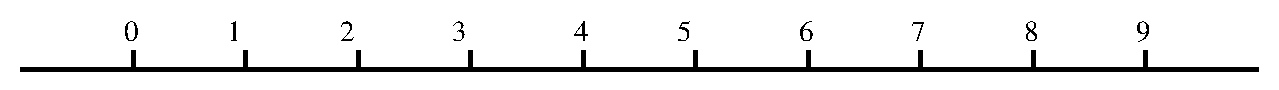
\includegraphics[width=0.6\textwidth]{xfig_stuff/Decimal_start.eps}
  \caption{Decimal numeral system.} 
  \label{fig:Decimal_start}
\end{figure}
It introduces the relation of order in our alphabet,
$$
0<1,\;1<2,\;2<3,\;3<4,\;4<5,\;5<6,\;6<7,\;7<8,\;8<9
$$
and we can lexicographically list all words that start with one of the letters from:\\
 $1,\;2,\;3,\;4,\;5,\;6,\;7,\;8,\;9.$
$$
1,\;2,\;3,\;4,\;5,\;6,\;7,\;8,\;9,\;10,\;11,\;12,\;13,\;14,\;15,\;\dots
$$  
%By applying our measuring stick again we put all those points onto the real line. Thus, we marked the set of natural numbers $\mathbb{N}.$ By prepending the metasymbol minus "$-$" to those names and also adding to our set $0$ we name the points on the left of $0$ and construct integers (Fig. ~\ref{fig:Decimal_integers}),
\begin{figure}[htbp]
  \centering
  \includegraphics[width=0.6\textwidth]{xfig_stuff/Decimal_integers.eps}
  \caption{Integers in decimal numeral system.} 
  \label{fig:Decimal_integers}
\end{figure}
$$
\mathbb{Z}=\{\dots,\;-4,\;-3,\;-2,\;-1,\;0,\;1,\;2,\;3,\;4,\;\dots\}
$$
Let $j\in \mathbb{Z}$ and $j\ge 0.$
 The names for points from the line consist of global and local addresses delimited by a metasymbol.
\begin{itemize} 
\item Points on the right of $0.$\\
\begin{enumerate}
\item Global address: the name for the integer $j,$ the left end of the interval.
\item Local address: the name of the point inside the interval  $[j,\;j+1).$ 
\end{enumerate}
\item Points on the left of $0.$\\
%On the other hand, each point from $(-(j+1),\;-j]$ has global and local addresses defined as follows. 
\begin{enumerate}
\item Global address: $-j,$ the right end of the interval.
\item Local address: the name of the point inside the interval  $(-(j+1),\;-j].$ 
\end{enumerate}
\end{itemize}
Local addresses are constructed in the same way as we did in binary and ternary numeral systems (see sections ~\ref{sec:binary}, ~\ref{sec:ternary}). The only difference is that we split intervals into ten equal parts labeled by  \href{https://en.wikipedia.org/wiki/Arabic_numerals_(disambiguation)}{Arabic numerals} $\{0,\;1,\;2,\;3,\;4,\;5,\;6,\;7,\;8,\;9\}.$ \\

By employing the technique from section ~\ref{sec:Euler-Fermat_algorithm} we illustrate the construction of a decimal address for a quotient with the following example. 

\begin{center}
\begin{picture}(60,1)
\thicklines
\put(0,0){\line(1,0){60}}
\end{picture}
\end{center}

\begin{example}
\label{ex:decimal}
We need to construct the digital representation for $\frac{64}{175} $ The calculations will be performed with the help of \href{https://github.com/mathhobbit/EditCalculateAndChart/releases}{EditCalculateAndChart}. First, the greatest common divisor $gcd(64,175)$ for $64$ and $175$ is equal to $1.$  The numbers $64$ and $175$ are coprime and the fraction $\frac{64}{175} $ is irreducible. In order to calculate $gcd(64,175)$ with \href{https://github.com/mathhobbit/EditCalculateAndChart/releases}{EditCalculateAndChart} you type it in the text area. Then highlight it with your mouse (Fig. ~\ref{fig:ECandC_gcd}). Clicking the calculator icon (the last in the tool bar) will calculate $gcd(64,175).$ 
\begin{figure}[htbp]
  \centering
  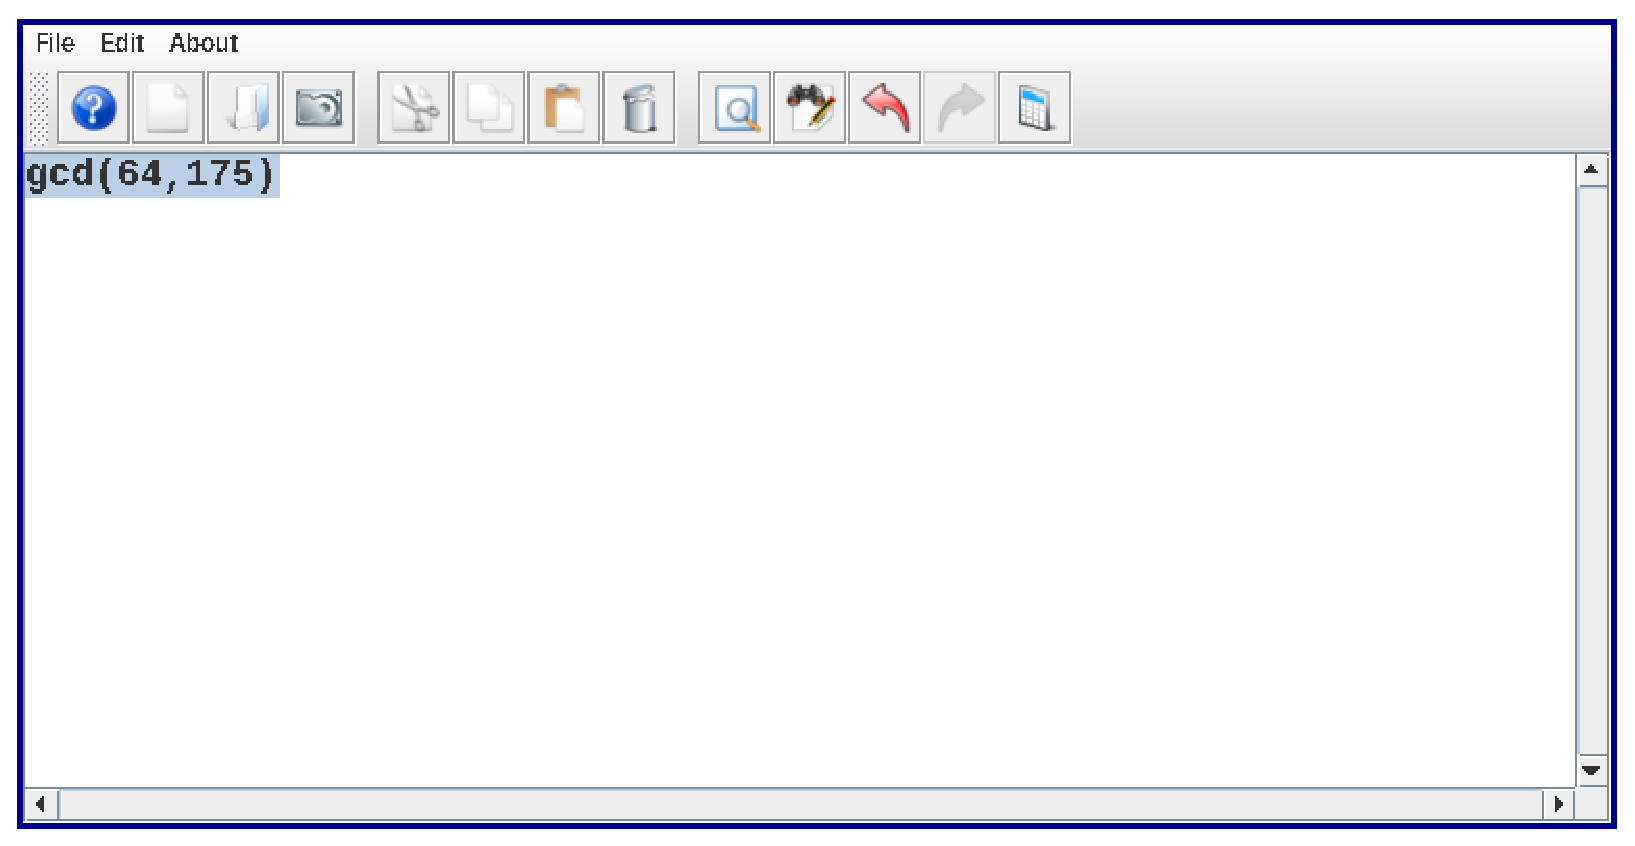
\includegraphics[width=0.6\textwidth]{image/ECandC_gcd.eps}
  \caption{Calculating $gcd(64,175).$} 
  \label{fig:ECandC_gcd}
\end{figure}
For radix $r=10$ and $n=175$ we will use Euler-Fermat algorithm (section ~\ref{sec:Euler-Fermat_algorithm}) to calculate natural numbers $q,\;\ell,\;s$ from Theorem ~\ref{th:Euler-Fermat}. \href{https://github.com/mathhobbit/EditCalculateAndChart/releases}{EditCalculateAndChart} has a procedure {\bf EF} which is an implementation of Euler-Fermat algorithm. One can get help in  \href{https://github.com/mathhobbit/EditCalculateAndChart/releases}{EditCalculateAndChart} by highlighting {\bf ?EF} and clicking the calculator icon (the last in the tool bar) (Fig. ~\ref{fig:ECandC_EF_help}).
\begin{figure}[htbp]
  \centering
  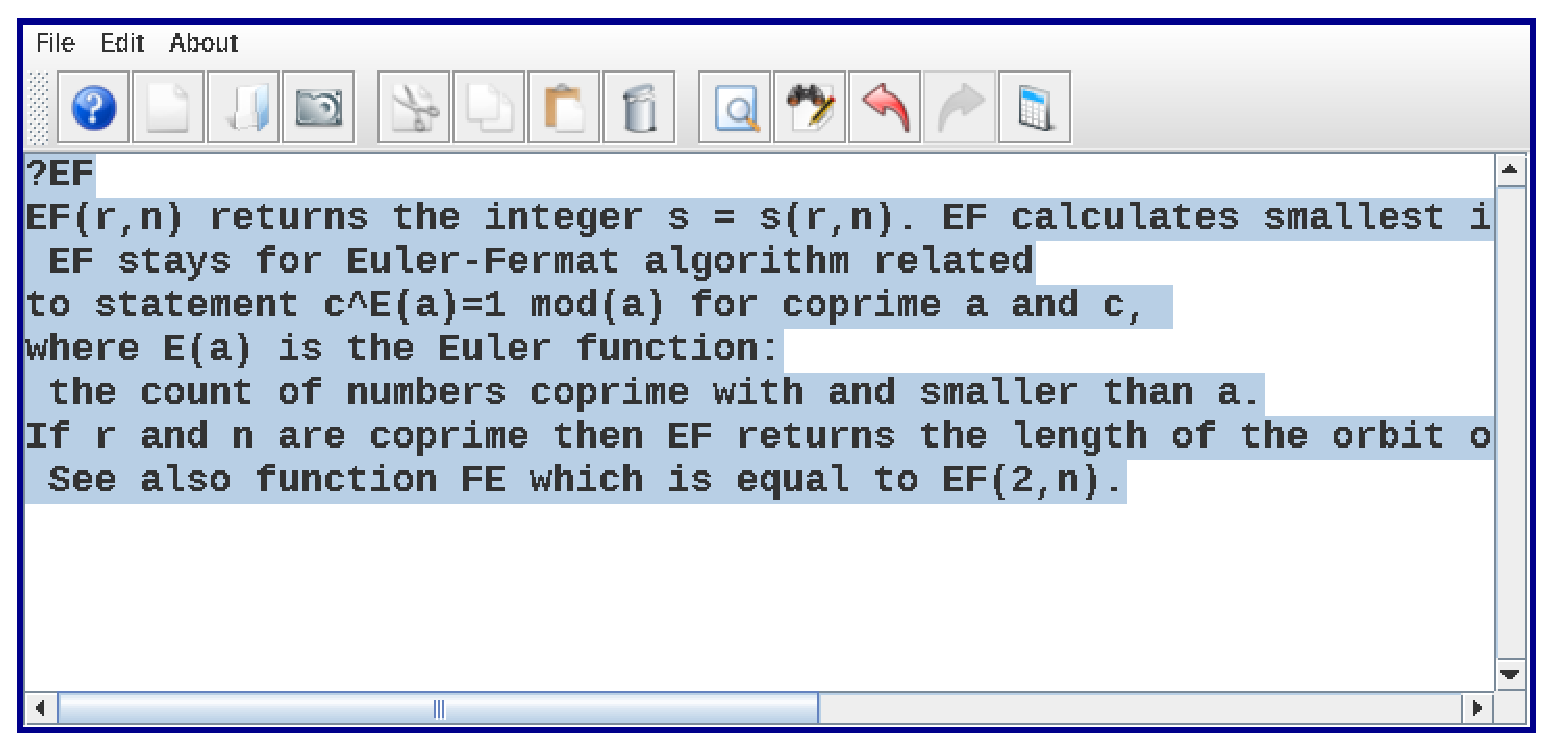
\includegraphics[width=0.6\textwidth]{image/ECandC_EF_help.eps}
  \caption{Help for {\bf EF}} 
  \label{fig:ECandC_EF_help}
\end{figure}
Highlighting {\bf EF(10,175)} and clicking the calculator button in  \href{https://github.com/mathhobbit/EditCalculateAndChart/releases}{EditCalculateAndChart} yields
$$
175\cdot 571428 = 10^2 \cdot (10^6-1)
$$
(Fig. ~\ref{fig:ECandC_EF}).
\begin{figure}[htbp]
  \centering
  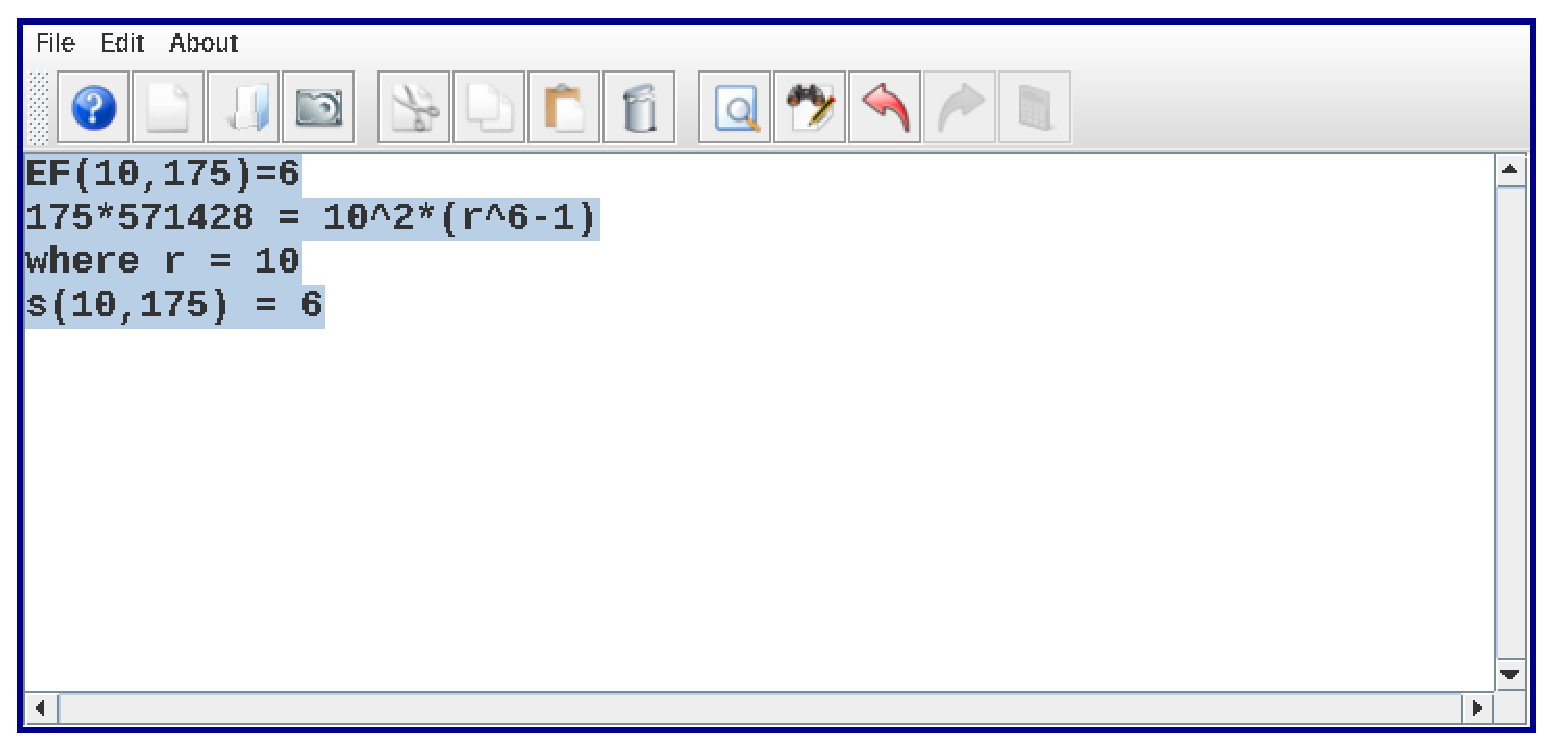
\includegraphics[width=0.6\textwidth]{image/ECandC_EF.eps}
  \caption{Calculating {\bf EF(10,175)}} 
  \label{fig:ECandC_EF}
\end{figure}
Thus,
$$
\frac{64}{175} = \frac{571428 \cdot 64}{571428  \cdot 175} =  \frac{571428 \cdot 64}{10^2 \cdot (10^6-1) }
$$
and
$$
\frac{571428 \cdot 64}{10^6-1} = 36 + \frac{571428}{10^6-1 }
$$
Hence,
$$
\frac{64}{175} = \frac{36}{10^2} + \frac{1}{10^2} \cdot \frac{5\cdot 10^5 + 7\cdot 10^4 + 1\cdot 10^3 + 4\cdot 10^2 + 2\cdot 10 + 8}{10^6} \cdot \sum_{j=0}^{\infty} \frac{1}{10^{6j}}
$$
We obtain the digital representation
$$
\frac{64}{175} = 0.36\overline{571428}
$$

\end{example}
\begin{center}
\begin{picture}(60,1)
\thicklines
\put(0,0){\line(1,0){60}}
\end{picture}
\end{center}

The denominator $175$  in Example ~\ref{ex:decimal} admits factorization $175 = 5^2 \cdot 7.$  One of its factors is $7.$ In Examples ~\ref{ex:ratios1} and ~\ref{ex:ratios2} the denominators also have $7$ as a prime factor. Considering decimal representations for ratios we observe that the prime number $7$ occupies a special place among  \href{https://en.wikipedia.org/wiki/Arabic_numerals_(disambiguation)}{Arabic numerals}  $\{0,\;1,\;2,\;3,\;4,\;5,\;6,\;7,\;8,\;9\}.$ In fact, if a power of $7^{\alpha }$ divides the denominator of a ratio $\frac{a}{b} \;\;(7^{\alpha } | b)$ then the length of the period for the decimal representation of  $\frac{a}{b}$ is greater or equal to $7^{\alpha -1 } \cdot 6.$ This fact can be added to the long list of "magic" properties of \href{https://en.wikipedia.org/wiki/7}{the magnificent seven $7$}: $7$ planets in the solar system, $7$ notes in music, etc.

\section{\href{https://en.wikipedia.org/wiki/Metric_space}{Metric space.} Limit. Topology. \href{https://en.wikipedia.org/wiki/Continuous_function}{Continuous function}. Completeness}
\label{sec:Metric}
The absolute value  of a real number $b$ is denoted by $|b|$ and defined as
$$
|b| = \max\{b,\;-b\}.
$$ 
Another competing definition for $|b|$ is
$$
|b| = \sqrt{b^2}
$$
where $\sqrt{b^2}$ denotes the positive solution for the equation
$$
x^2 = b^2
$$
where $x$ is unknown.\\

The distance between real numbers $a,\;b\in \mathbb{R}$ is defined as $|b-a|.$ The absolute value function $|x|$ maps the real line $\mathbb{R}$ into the set of non-negative real numbers (those on the right of $0$ with $0$ included),
$$
\mathbb{R}_+ = \{x\in \mathbb{R},\;x\ge 0 \}
$$ 
The set of real numbers $\mathbb{R}$ together with the absolute value function $|x|$ becomes \href{https://en.wikipedia.org/wiki/Metric_space}{a metric space}. In order to introduce the concept of a metric space we need \href{https://en.wikipedia.org/wiki/Cartesian_product}{Cartesian product}.
\begin{definition} (Cartesian product)\\
\label{def:Cartesian}
Given sets $A$ and $B$ 
$$
A\times B = \{(a,b),\;\;a\in A,\; b\in B\}
$$ 
is called Cartesian product of $A$ and $B.$
\end{definition}
Now we are ready for a metric space definition.
\pagebreak
\begin{definition} (Metric space)\\
\label{def:SpaceMetric}
A set $M$ together with the function $d(x,y)$ (the distance from $x$ to $y),$
$$
d:\;\;M \times M \;\to \; \mathbb{R}_+
$$
is called \href{https://en.wikipedia.org/wiki/Metric_space}{a metric space} if the following is true for all $x,\;y,\;z\in M.$ 
\begin{itemize}
\item[] $d(x,x) = 0$ \href{https://en.wikipedia.org/wiki/Reflexive_relation}{(reflexivity).}
\item[] $d(x,y)=d(y,x)$ (symmetricity).
\item[] $d(x,z)\le d(x,y)+d(y,z)$ (triangle property).
\end{itemize}
\end{definition}
For the real line $\mathbb{R}$ the distance function
$$
d(x,y) = |x-y|.
$$
In order to show that $\mathbb{R}$ is a metric space we need to prove that $|x-y|$ possesses reflexivity, symmetricity and triangle property. The proof of reflexivity and symmetricity is left as an exercise for the reader. It is a bit tricky to see that the triangle property is valid for $|x-y|.$ 
Note that 
$$
|x| = \max\{-x,x\}
$$
implies 
\begin{eqnarray*}
x &\le & |x|\\ 
-x &\le & |x|
\end{eqnarray*}  
which is equivalent to
$$
-|x| \le x \le |x|.
$$
If follows from
\begin{eqnarray*}
&& -|a| \le a \le |a|\\
+&&\\
&&-|b| \le b \le |b|\\
&&\overline{-|a| - |b| \le a + b \le  |a| +|b|}
\end{eqnarray*}
that
$$
|a+b| \le |a| + |b|.
$$
Setting $a=x-y$ and $b=y-z$ we have
$$
|x-z| = |x-y + y-z| \le |x-y|+ |y-z|
$$
and triangle property follows.\\
A sequence is a list of real numbers written next to each other,
$$
\{s(j)\}_{j=1}^{\infty} = \{ s(1),\;s(2),\;\dots \}
$$ 
Sequences appear in many real world applications: the sequence of prices of a financial instrument (economics, investment), measurements of temperature for a patient (medicine), numbers of sun spots (solar activity) etc.\\
Every sequence is associated with a function
$$
s:\;\mathbb{N} \to \mathbb{R}
$$
In order to study properties of sequences we introduce the graph $G_s \subset \mathbb{R}^2$ of a sequence $\{s(n)\}_{n=1}^{\infty}$ defined as follows.
$$
G_s = \{(n,\;s(n));\; n\in \mathbb{N}\}
$$
Let us illustrate the concept of the graph with examples.
\begin{center}
\begin{picture}(60,1)
\thicklines
\put(0,0){\line(1,0){60}}
\end{picture}
\end{center}
\begin{example}
\label{ex:sequence1}
Consider the sequence
$$
s=\{1+\frac{(-1)^n}{n}\}_{n=1}^{\infty}
$$
The first $20$ points from its graph are depicted on Fig. ~\ref{fig:sequence1}. It is done with \href{https://github.com/mathhobbit/EditCalculateAndChart/releases}{EditCalculateAndChart} (Fig. ~\ref{fig:sequence2}). In the study of sequences we do not care about the first $n$ points of a sequence regardless of how big $n$ is. The behavior of the sequence is defined by its tail $\{s(n)\}_{n=k}^{\infty},$ where $k$ is any natural number (the bigger the better).
 It is all about tails as far as sequences concerned. For this reason when  we study a tail of a sequence  $\{s(n)\}_{n=1}^{\infty}$ we simply write
$$
  \{s(n)\}
$$
because $n=1$ in $\{s(n)\}_{n=1}^{\infty}$ is not important and $\infty$  is self evident.
 In order to guess the behavior for the tail of our sequence we plot $100$ points from the sequence graph together with their projections on $y$-axis.  \href{https://github.com/mathhobbit/EditCalculateAndChart/releases}{EditCalculateAndChart} procedure for that is presented on Fig. ~\ref{fig:sequence3} and the result of its execution is on Fig. ~\ref{fig:sequence4}. By looking at ~\ref{fig:sequence4} we can see that the points from the sequence tail are densely packed near the point $1$ on $y$-axis. The point $1$ is called \href{https://en.wikipedia.org/wiki/Dense_set}{the limit point (dense point)} of the sequence.
\begin{figure}[htbp]
  \centering
  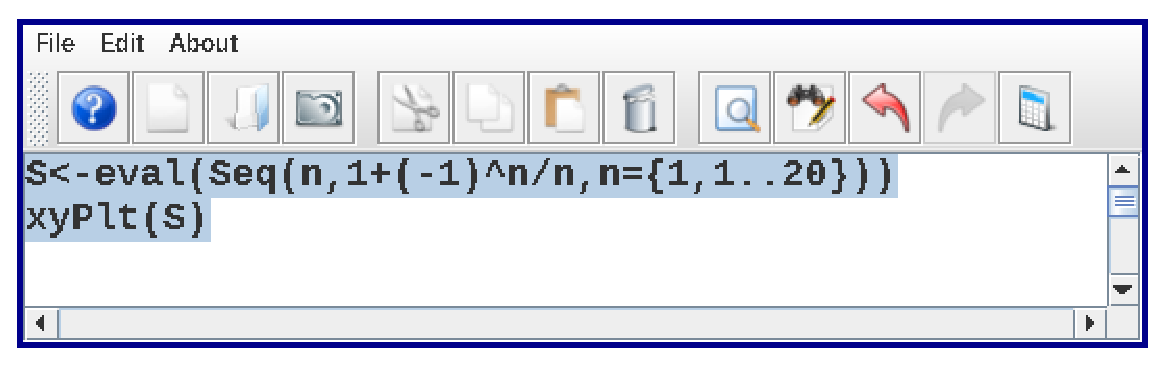
\includegraphics[width=0.6\textwidth]{image/sequence2.eps}
  \caption{Plotting the first 20 points of $\{(n,1+\frac{(-1)^n}{n})\}_{n=1}^{\infty}$}
  \label{fig:sequence2}
\end{figure}
\begin{figure}[htbp]
  \centering
  \includegraphics[width=0.6\textwidth]{image/sequence1.png}
  \caption{The first $20$ points of $\{(n,1+\frac{(-1)^n}{n})\}_{n=1}^{\infty}$}
  \label{fig:sequence1}
\end{figure}
\begin{figure}[htbp]
  \centering
  \includegraphics[width=0.6\textwidth]{image/sequence3.eps}
  %\caption{Plotting the first 100 points of $\{(n,1+\frac{(-1)^n}{n})\}_{n=1}^{\infty}$ together with their projections on $y$-axis.}
  \caption{Plotting points of the sequence graph together with their projections on $y$-axis.}
  \label{fig:sequence3}
\end{figure}
\begin{figure}[htbp]
  \centering
  \includegraphics[width=0.6\textwidth]{image/sequence4.png}
  \caption{The first $100$ points of $\{(n,1+\frac{(-1)^n}{n})\}_{n=1}^{\infty}$ together with their projections on $y$-axis.}
  \label{fig:sequence4}
\end{figure}
\end{example}
\begin{center}
\begin{picture}(60,1)
\thicklines
\put(0,0){\line(1,0){60}}
\end{picture}
\end{center}
The sequence from example ~\ref{ex:sequence1} has the limit equal to $1.$ For the formal definition of the limit we need the concept of topology, the open set and neighborhood of a point.
\begin{definition}
(Topology)\\
A topology $\tau $ on a set $X$ is defined by a family $\tau $ of subsets from $X.$ This family $\tau$ is to meet the following requirements.
\begin{enumerate}
\item Empty set $\emptyset$ and $X$ belong to $\tau;$  $\emptyset \in \tau,\;\;X \in \tau.$
\item Let $A$ be an arbitrary set of indices. If
$$
\forall \alpha \in A\;\;\;S_{\alpha } \in \tau
$$
then
$$
\bigcup_{\alpha \in A} S_{\alpha } \in \tau
$$
\item Given $n \in \mathbb{N}$ if
$$
S_j \in \tau \;\;\mbox{ for }\;\;j=1,\;2,\dots \;n
$$
then
$$
\bigcap_{j=1}^{n} S_j \in \tau
$$
$\tau$ is called the family of open (sub)sets from $X.$ A set S is called open (in topology $\tau$) if $S\in \tau .$
\end{enumerate}
\end{definition}
Consider two topologies $\tau_1$ and $\tau_2$ on $X$ such that $\tau_1 \subset \tau_2$ then we are saying that the topology $\tau_1$ is \href{http://mathonline.wikidot.com/weaker-and-stronger-topologies}{weaker (coarser)} than $\tau_2$  or $\tau_2$ is \href{http://mathonline.wikidot.com/weaker-and-stronger-topologies}{stronger} (finer) than $\tau_1.$ The weakest topology on $X$ is $\tau_0 = \{\emptyset,\; X\}.$ The strongest topology on $X$ is defined by $\tau_{\infty}$ that includes all possible subsets from $ X.$ All other topologies on X are sitting in between of $\tau_0$ and $\tau_{\infty}.$
\begin{center}
\begin{picture}(60,1)
\thicklines
\put(0,0){\line(1,0){60}}
\end{picture}
\end{center}
\begin{example}
Consider a set $X$ that has only two elements $A$ and $B.$ We can define four different topologies on $X.$ The weakest topology
$$
\tau_0=\{\emptyset,\; X\}.
$$
The strongest
$$
\tau_{\infty}=\{\emptyset,\;A,\;B,\; X\}
$$
where $A$ denotes the set that has only one element $A$ and so is $B.$\\
There are two topologies in between of $\tau_0$ and $\tau_{\infty}$.
$$
\tau_1= \{\emptyset,\;A,\; X\}\;\;\mbox{ and } \tau_2= \{\emptyset,\;B,\; X\}.
$$
Note that in terms of stronger/weaker $\tau_1$ and $\tau_2$ are incomparable.
\end{example}
\begin{center}
\begin{picture}(60,1)
\thicklines
\put(0,0){\line(1,0){60}}
\end{picture}
\end{center}
\begin{definition}
\label{def:neighborhood}
(Open set, neighborhood)\\
Given two points $a,\;b\in \mathbb{R}$ the open interval $(a,\;b)$ is defined as
$$
(a,\;b) =\{x\in \mathbb{R},\;a<x<b\}
$$
All open intervals from $\mathbb{R}$ define \href{https://en.wikipedia.org/wiki/Base_(topology)}{a base (or basis)} for the topology of real line $\mathbb{R}.$ In other words, a subset of $\mathbb{R}$ is open if, and only if, it is a union of open intervals.\\
An open neighborhood of a point $p\in \mathbb{R}$ is an open set $S$ such that $p \in S.$
\end{definition}
According to Definition ~\ref{def:neighborhood} any open interval $(a,\;b)$ can serve as an open neighborhood of $p\in\mathbb{R}$ as long as 
$$
p \in (a,\;b)\;\;\mbox{ or } \;\;a<p<b.
$$
\begin{definition}
\label{def:limit}
(Limit)\\
%A point $L\in \mathbb{R}$ is a limit of a sequence $\{s(n)\}$ if, and only if, any neighborhood of $L$ conatins all elements of $\{s(n)\}$ but a few finitely many members, outsiders from $\{s(n)\}.$ Then we write
Regardless of  an open neighborhood $U$ of $L\in \mathbb{R}$ \textcolor{red}{EVERYBODY} is in $U$ but only few (finitely many) are out of $U,$ as far as members of the sequence  $\{s(n)\}$ concerned. Then we are saying that $L$ is the limit of the sequence  $\{s(n)\}$ and writing
$$
\;\;\lim_{n\to \infty} \; s(n) \; =\; L, \;\;\mbox{ or }\;\;\lim \;s(n) \;=\; L\;\;\;\mbox{ or } \;\;s(n) \to L
$$ 
\end{definition}
For sequences it is kind of excessive to write $n\to \infty$ under the sign of the limit. So we skip $n \to \infty $ when we are talking about sequences.
\begin{definition}
\href{https://en.wikipedia.org/wiki/Continuous_function}{(Continuous function)}
Consider a real function 
$$
f:\;\mathbb{R} \to \mathbb{R}
$$
Let $p\in \mathbb{R}$ and $f(p)$ be defined. If for any sequence $\{s(n)\}$ 
$$
s(n) \to p
$$
yields
$$
f(s(n)) \to f(p)
$$
then $f(x)$ is called \href{https://en.wikipedia.org/wiki/Continuous_function}{continuous} at $p.$ 
\end{definition}


 The next statement follows immediately from Definition ~~\ref{def:limit}.
\begin{theorem}
Let
$$
a(n) \to A\;\;\;\;\mbox{ and }\;\;\;\;b(n) \to B,
$$ 
where $A,\;B\in \mathbb{R}.$
Then
\begin{enumerate}
\item (Limit of the sum is the sum of the limits)\\
$\lim (\alpha \cdot a(n) + \beta \cdot b(n)) = \alpha \cdot \lim a(n) +  \beta \cdot  \lim b(n),$ where $\alpha ,\;\beta \in \mathbb{R}$
\item (Limit of the product (ratio) is the product (ratio) of the limits.)\\
$\lim a(n)\cdot b(n) = \lim a(n) \cdot \lim b(n)$\\
$\lim \frac{a(n)}{b(n)} =  \frac{\lim a(n)}{ \lim b(n)}$ as long as it makes sense, id est $\lim b(n) \not= 0.$
\item If a real function is continuous at $A$ then
$$
\lim f(a(n)) = f(\lim a(n))
$$
\item (\href{https://en.wikipedia.org/wiki/Squeeze_theorem}{Squeeze theorem})\\
Consider sequences $\{a(n)\},\;\{b(n)\}$ and $\{c(n)\}$ such that
$$
a(n) \le b(n) \le c(n)\;\;\;\mbox{ and }\;\;\; \lim a(n) = \lim c(n) 
$$
Then
$$
\lim b(n) = \lim a(n) = \lim c(n) 
$$
\end{enumerate}
\end{theorem}


  \textcolor{red}{EVERYBODY} is essential for the concept of limit (Definition ~\ref{def:limit}). It makes limit unique for a sequence if the sequence has the limit. However, a sequence might not have a limit but instead might have several limit (or dense) points defined as follows.
\begin{definition}
(Limit (dense) point)\\
Regardless of  an open neighborhood $U$ of $L\in \mathbb{R}$ \textcolor{red}{infinitely many} members of $\{s(n)\}$ are in $U.$ Then we are saying that $L$ is the limit (dense) point of the sequence  $\{s(n)\}.$ 
\end{definition}
If one mixes together several sequences having different limits then the result will be a sequence with several limit (dense) points that does not have a limit.
\begin{center}
\begin{picture}(60,1)
\thicklines
\put(0,0){\line(1,0){60}}
\end{picture}
\end{center}
\begin{example}
Consider a sequence 
$$
\{(-1)^n+\frac{1}{n}\}
$$
It is a mixture of 
$$
\{-1+\frac{1}{n}\} \mbox{  and  } \{1+\frac{1}{n}\}
$$
The sequence $\{(-1)^n+\frac{1}{n}\}$ does not have a limit. However, it has two limit points, $-1$ and $1$ (Fig. ~\ref{fig:sequece_2_limit_points}).
\begin{figure}[htbp]
  \centering
  \includegraphics[width=0.6\textwidth]{image/sequece_2_limit_points.png}
  \caption{The first $100$ points of $\{(n,(-1)^n+\frac{1}{n})\}_{n=1}^{\infty}$ together with their projections on $y$-axis.}
  \label{fig:sequece_2_limit_points}
\end{figure}
\end{example}
\begin{center}
\begin{picture}(60,1)
\thicklines
\put(0,0){\line(1,0){60}}
\end{picture}
\end{center}
The next example presents a sequence that has infinitely many limit points.
\begin{center}
\begin{picture}(60,1)
\thicklines
\put(0,0){\line(1,0){60}}
\end{picture}
\end{center}
\begin{example}
Consider
$$
\{\sin(n)\}_{n=1}^{\infty}
$$
Plotting the first $1500$ points of the sequence graph (see Fig. ~\ref{fig:sequece_infinit_limit_points}) supports our guess about infinitely many limit points for $\{\sin(n)\}.$
\begin{figure}[htbp]
  \centering
  \includegraphics[width=0.6\textwidth]{image/sequece_infinit_limit_points.png}
  \caption{The first $1500$ points of $\{(n,\sin(n)\}_{n=1}^{\infty}$ together with their projections on $y$-axis.}
  \label{fig:sequece_infinit_limit_points}
\end{figure}
\end{example}
\begin{center}
\begin{picture}(60,1)
\thicklines
\put(0,0){\line(1,0){60}}
\end{picture}
\end{center}
If  a sequence $\{s(n)\}$ has a limit $L\in \mathbb{R},$ 
$$
\lim\;s(n) \;=\; L
$$
then
$$
\forall \varepsilon \in \mathbb{R},  \;\;\; \varepsilon >0\;\;\exists\;\;K\in \mathbb{N}\;\;\mbox{ such that }\;\;\forall\;\;n>K\;\;\;|s(n) - L| < \varepsilon 
$$
Hence,
$$
\forall \varepsilon \in \mathbb{R},  \;\;\; \varepsilon >0\;\;\exists\;\;K\in \mathbb{N}
$$
such that $\forall\;\;n>K$ and $m>K$
\begin{eqnarray*}
&&- \varepsilon < s(n) - L < \varepsilon\\
+&&\\
&&- \varepsilon <  L - s(m) < \varepsilon\\
&&\overline{-2 \cdot \varepsilon  < s(n)-s(m) < 2\cdot \varepsilon}
\end{eqnarray*}
Therefore,
$$
\forall \varepsilon \in \mathbb{R},  \;\;\; \varepsilon >0\;\;\exists\;\;K\in \mathbb{N}\;\;\mbox{ such that }\;\;\forall\;\;n>K,\;\;m>K\;\;\;|s(n) - s(m)| < 2\cdot \varepsilon 
$$
The sequence with such property is called \href{https://en.wikipedia.org/wiki/Cauchy_sequence}{a Cauchy sequence.} One can define a Cauchy sequence in any metric space $M$ with a distance $d.$
\begin{definition} (Cauchy sequence)\\
Let $\{s(n)\}$ be a sequence in a metric space $M$ with distance $d.$ Then $\{s(n)\}$  is a Cauchy sequence in $M$ if, and only if,
$$
\forall \varepsilon \in \mathbb{R},  \;\;\; \varepsilon >0\;\;\exists\;\;K\in \mathbb{N}\;\;\mbox{ such that }\;\;\forall\;\;n>K,\;\;m>K\;\;\;d(s(n) , s(m)) <  \varepsilon 
$$
\end{definition}
A sequence $\{s(n)\}$ in a metric space $M$ with distance $d$ is called bounded if  
$$
\exists p\in X\;\;\mbox{ and } B\in \mathbb{R}_{+}\;\;
$$
such that for all members of the sequence $\{s(n)\}$ the following takes place.
$$
d(p,s(n))<B.
$$
In particular, a sequence $\{s(n)\}$ from $\mathbb{R}$ is bounded if, and only if,
$$
\exists (a,\;b) \subset \mathbb{R}_{+} \;\;\mbox{ such that } s(n) \in (a,\;b) 
$$
for all $s(n)$ from $\{s(n)\}.$ It is left for the reader as an exercise to prove that every Cauchy sequence is bounded.

\begin{definition} (Completeness)\\
A metric space $M$ is complete if, and only if, its every Cauchy sequence has a limit from $M.$
\end{definition}
Real numbers $\mathbb{R}$ is a complete metric space with the distance function $d(a,b)=|a-b|.$  It follows from the following statement.
\begin{theorem}
\label{th:completeness}
Every bounded sequence in  $\mathbb{R}$  has a limit point from $\mathbb{R}.$

\end{theorem} 
\begin{proof}
Note that given $a,\;b \in \mathbb{R}$ mapping
$$
\mu_{a,b}(x) = \frac{x-a}{b-a}
$$
is a one-to-one mapping 
$$
\mu_{a,b}:\;\mathbb{R} \;\to \;\mathbb{R}
$$
If $b>a$ then
$$
\mu_{a,b}:\;[a,\;b] \; \to \; [0,\;1]
$$
The inverse $\mu_{a,b}^{-1}$ of $\mu_{a,b}$ is
$$
\mu_{a,b}^{-1}(x) = (b-a) \cdot x+a 
$$
and
$$
\mu_{a,b}^{-1} :\;  [0,\;1] \to \;[a,\;b].
$$ 
Consider a bounded sequence $\{s(n)\}$ from $\mathbb{R}.$ There exists an open interval $(a,\;b)$ such that $ s(n) \in (a,\;b)$ for all $s(n)$ from $\{s(n)\}.$ The sequence $\{\mu_{a,b} (s(n)) \}$ belong to $(0,1).$ \href{https://en.wikipedia.org/wiki/Without_loss_of_generality}{Without loss of generality} we assume that $\{\mu_{a,b} (s(n)) \}$ has infinitely many members.\\
Let us use binary numeral system (section \ref{sec:binary}) in order to construct a limit point $p\in (0,\;1)$ for $\{\mu_{a,b} (s(n)) \}.$ We divide the interval $(0,\;1)$ into two equal parts. The first part we call $0$ the second $1.$ We choose the part with infinitely many members of  $\{\mu_{a,b} (s(n)) \}.$ Its name (either $0$ or $1)$ will be the first letter of the local address for $p.$ Then we split the chosen part into two equal parts $0$ and $1.$ Pick the one with infinitely many members of $\{\mu_{a,b} (s(n)) \}.$ Its name will be the second letter of the local address for $p.$   Continue in this manner (Fig. ~\ref{fig:completeness}) we find the local address for $p.$ By construction $p$ is a limit point for $\{\mu_{a,b} (s(n)) \}$  because every open neighborhood of $p$ has infinitely many members of $\{\mu_{a,b} (s(n)) \}.$ Hence, $\mu_{a,b}^{-1}(p)$ is a limit point for $\{s(n)\}.$
 
\begin{figure}[htbp]
  \centering
  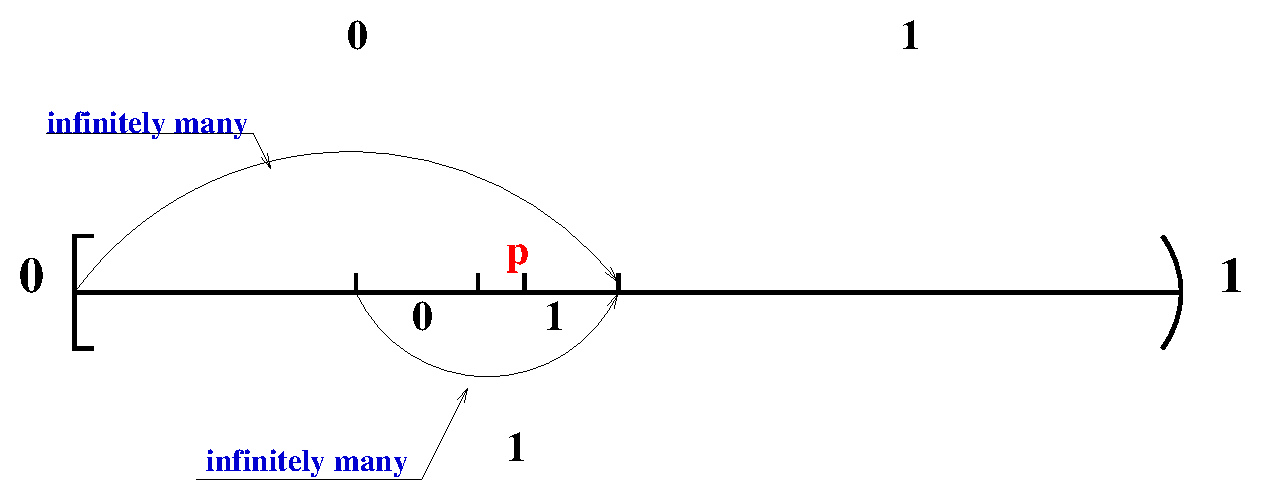
\includegraphics[width=0.6\textwidth]{xfig_stuff/completeness.eps}
  \caption{\textcolor{red}{p}$=0.011\dots$ is a limit point.}
  \label{fig:completeness}
\end{figure}
\vspace{0.1cm}
Q.E.D.
\vspace{0.1cm}
\end{proof}

It follows from Theorem ~\ref{th:completeness} that $\mathbb{R}$ is complete. Because  every Cauchy sequence from $\mathbb{R}$ is bounded and has the only limit point from $\mathbb{R}$ which is the limit of the Cauchy sequence. 






%%%%%%%%%%%%%%%%Conclusion
\phantomsection
%\addcontentsline{toc}{chapter}{Conclusion}
\section*{Conclusion}
A few words before we part, if you get here after reading everything above then it is time to care for your psychological well-being. After completing this text you know real numbers a bit better then your classmates and also probably better than some of your instructors. Please have mercy on them, they also are victims of the educational system like you and I. Do not show you superiority at any circumstances. Instead try to help them to gain the knowledge that you already have.
%%%%%%%%%%%%%%%%%%%done with conclusion

%\section{\href{https://en.wikipedia.org/wiki/Minkowski_space}{Minkowski space}}
%SergeY
%\printindex
\end{document}
